\documentclass[12pt,a4]{report}
\usepackage{textcomp}
\usepackage{fancyhdr}
\usepackage{graphicx}
\usepackage{titletoc,tocloft}
\usepackage{enumitem}
\usepackage{amsmath,amssymb}
\evensidemargin 0.5in
\oddsidemargin 0.0in
\topmargin 0.5in
\textwidth 6.5in
\headheight 0.3in
\headsep 0in
\usepackage[]{hyperref}
\usepackage{tikz}
\usetikzlibrary{arrows,shapes,snakes,automata,backgrounds,petri}
\usepackage{tabularx}
\usepackage{pgfgantt}
\usepackage[margin=1in]{geometry}
\usepackage{lscape}
\usepackage{array}
\usepackage{longtable}
\usepackage{multirow}
\usepackage[titletoc]{appendix}
\renewcommand{\bibname}{References}
\setcounter{secnumdepth}{5}
\usepackage{float}
\usepackage{subcaption}
\usepackage{multirow}
\usepackage{longtable}
\usepackage{geometry}
\geometry{margin=1in}
\usepackage{caption}
\usepackage{tocloft}
\usepackage[ruled,vlined]{algorithm2e}
\newcommand{\cellpadding}{\renewcommand{\arraystretch}{1.2}}
\newcommand{\headerpadding}{\renewcommand{\arraystretch}{1.5}}
\newcolumntype{P}[1]{>{\raggedright\arraybackslash}p{#1}}
\textheight 8.5in
\newcommand{\pa}{\hspace{3ex}}
\newcommand{\be}{\begin{equation}}
\newcommand{\ee}{\end{equation}}
\newcommand{\fs}{\hspace{2ex}}
\newcommand{\no}{\noindent}
\newcommand{\hs}{\hspace{1ex}}
\newtheorem{myth}{Theorem}
\newcommand{\smci}{{\bf smci }}
\newcommand{\smcd}{{\bf smcd }}
\newcommand{\smc}{{\bf smc }}
\newcommand{\ab}{{\bf sc4c }}
\newcommand{\hub}{H\"ubler }
\newcommand{\ds}{D^m_f}
\newtheorem{prop}{Proposition}
\newtheorem{cor}{Corollary}
\newtheorem{defn}{Definition}
\newcommand{\rr}{{\cal R }^2 }
\newcommand{\zz}{{\cal Z }^2 }
\newcommand{\at}{{A_o}^T}
\newcommand{\ato}{{A_1}^T}
\newcommand{\ath}{{\at}_{\hat{h}}}
\newcommand{\ata}{\tilde{\at}}
\newcommand{\on}{(s_1,\hat{s_1}]}
\newcommand{\tw}{(\hat{s_1},b]}
\newcommand{\hb}{\hat{B}}
\newcommand{\hfo}{{\hat{f}}_1}
\newcommand{\xy}{(x,y)}
\newcommand{\txy}{(t_x,t_y)}
\renewcommand{\r}{{\cal R}}
\newcommand{\ct}{\hat{C}_1^T}
\newcommand{\xh}{X_{\hat{h}}}
\newcommand{\ball}{B((x_o,y_o),r)}
\newcommand{\snbd}{S((x_o,y_o),k)}
\newcommand{\xyo}{(x_o,y_o)}
\newtheorem{obs}{Observation}
\newtheorem{lemma}{Lemma}
\newcommand{\CC}{{\cal C }}
\newcommand{\DD}{{\cal D }}
\newcommand{\cset}{{\{C\}}}
\newcommand{\dset}{{\{D\}}}
\newcommand{\sdset}{{\sigma_{\dset}}}
\newcommand{\dsetm}{{m\dset}}
\newcommand{\sdsetm}{{\sigma_{\dsetm}}}
\newcommand{\od}{{O_D}}
\newcommand{\id}{{I_D}}
\newcommand{\ido}{{\id_1}}
\newcommand{\idt}{{\id_2}}
\newcommand{\odo}{{\od_1}}
\newcommand{\odt}{{\od_2}}
\newcommand{\rido}{{R(\ido)}}
\newcommand{\ridt}{{R(\idt)}}
\newcommand{\rodo}{{R(\odo)}}
\newcommand{\rodt}{{R(\odt)}}
\newcommand{\xe}{$x$-extent}
\newcommand{\ye}{$y$-extent}
\newcommand{\kxo}{k_{x1}}
\newcommand{\kxt}{k_{x2}}
\newcommand{\kxth}{k_{x3}}
\newcommand{\kyo}{k_{y1}}
\newcommand{\kyt}{k_{y2}}
\newcommand{\kyth}{k_{y3}}
\newcommand{\Ra}{{\Rightarrow}}
\newcommand{\is}{\Rightarrow \hspace{10mm}}
\newcommand{\vs}{\vspace{0.2in}}
\newcommand{\im}{{\lfloor m \rfloor}}
\newcommand{\fm}
\newcommand{\dm}{{\Delta m}}
\newcommand{\ic}{{\lfloor c \rfloor}}
\newcommand{\fc}
\newcommand{\dc}{{\Delta c}}
\newcommand{\yi}{{y_i}}
\renewcommand{\xi}{{x_i}}
\newcommand{\alpp}{{{\alpha}_{2}}}
\newcommand{\alp}{{{\alpha}_{1}}}
\newcommand{\bett}{{{\beta}_{2}}}
\newcommand{\bet}{{{\beta}_{1}}}
\newcommand{\lqr}{{\lfloor q \rfloor}}
\newcommand{\ramax}{R_{max}^A}
\newcommand{\ramin}{R_{min}^A}
\newtheorem{property}{Property}
\newcommand{\sla}{{{S_{\lambda}}}}
\newcommand{\vf}{{\vspace{0.50in}}}
\newcommand{\ms}{\;}
\renewcommand{\appendixname}{Annexure}

% Define counters for modules, submodules, and sub-submodules
\newcounter{lofmodule}
\newcounter{lofsubmodule}[lofmodule]
\newcounter{lofsubsubmodule}[lofsubmodule]

% Reset lower counters when higher-level increments
\renewcommand{\thelofmodule}{\arabic{lofmodule}}
\renewcommand{\thelofsubmodule}{\thelofmodule.\arabic{lofsubmodule}}
\renewcommand{\thelofsubsubmodule}{\thelofsubmodule.\arabic{lofsubsubmodule}}

% Command for List of Figures module (level 1)
\newcommand{\lofsection}[1]{%
  \refstepcounter{lofmodule}%
  \setcounter{lofsubmodule}{0}%
  \setcounter{lofsubsubmodule}{0}%
  \addtocontents{lof}{\protect\vspace{1em}}%
  \addtocontents{lof}{\protect\noindent \textbf{\thelofmodule.\hspace{1em} #1}\protect\par}%
  \addtocontents{lof}{\protect\vspace{0.5em}}%
}

% Command for List of Figures submodule (level 2)
\newcommand{\lofsubsection}[1]{%
  \refstepcounter{lofsubmodule}%
  \setcounter{lofsubsubmodule}{0}%
  \addtocontents{lof}{\protect\vspace{0.5em}\noindent \textbf{\thelofsubmodule.\hspace{1em} #1}\protect\par}%
}

% Command for List of Figures sub-submodule (level 3)
\newcommand{\lofsubsubsection}[1]{%
  \refstepcounter{lofsubsubmodule}%
  \addtocontents{lof}{\protect\noindent \hspace{0em}\textbf{\thelofsubsubmodule.\hspace{1em}\vspace{0.5em} #1}\protect\par}%
}
\renewcommand{\contentsname}{INDEX}

\fancypagestyle{chaptertitle}{
  \fancyhf{} % clear all
  \renewcommand{\headrulewidth}{0pt}
  \renewcommand{\footrulewidth}{0pt}
}

\makeatletter
\def\@makechapterhead#1{%
  \vspace*{\fill}%
  \begin{center}
    {\Huge\bfseries CHAPTER \thechapter\\[1.5ex]#1}
  \end{center}
  \thispagestyle{chaptertitle}% 
  \vspace*{\fill}
  \clearpage
}
\def\@makeschapterhead#1{%
  \vspace*{\fill}%
  \begin{center}
    {\Huge\bfseries #1}
  \end{center}
  \thispagestyle{chaptertitle}%
  \vspace*{\fill}
  \clearpage
}
\makeatother

\newcommand{\createGanttChart}{%
    \begin{table}[htbp]
    \centering
    \begingroup
    \renewcommand\sfdefault{phv}
    \renewcommand\mddefault{mc}
    \renewcommand\bfdefault{bc}
    
    \sffamily
    \begin{ganttchart}[
        % --- Chart Styling ---
        canvas/.append style={fill=none, draw=black!5, line width=.75pt},
        hgrid style/.style={draw=black!5, line width=.75pt},
        vgrid={*1{draw=black!5, line width=.75pt}},
        title/.style={draw=none, fill=none},
        title label font=\bfseries\footnotesize,
        title label node/.append style={below=7pt},
        include title in canvas=false,
        bar label font=\mdseries\small\color{black!70},
        bar label node/.append style={left=2cm},
        bar/.append style={draw=none, fill=black!63},
        bar incomplete/.append style={fill=barblue},
        bar progress label font=\mdseries\footnotesize\color{black!70},
        group incomplete/.append style={fill=groupblue},
        group left shift=0,
        group right shift=0,
        group height=.5,
        group peaks tip position=0,
        group label node/.append style={left=.6cm},
        group progress label font=\bfseries\small,
        x unit=0.7cm,
        title label node/.append style={xshift=0.1cm}
    ]{1}{12}
      % --- Titles ---
      \gantttitle[
        title label node/.append style={below left=7pt and -3pt}
      ]{A.Y. 2025-2026}{12} \\
      \gantttitlelist[
        title label node/.append style={below left=7pt and -3pt}
      ]{{"Nov"}, {"Dec"}, {"Jan"}, {"Feb"}, {"Mar"}, {"Apr"}, {"May"}, {"Jun"}, {"Jul"}, {"Aug"}, {"Sep"}, {"Oct"}}{1} \\
      % --- Tasks ---
      \ganttgroup{Project Timeline}{1}{12} \\
      \ganttbar[name=planning]{\textbf{1.} Planning, Requirement Gathering \& Literature Survey}{1}{3} \\
      \ganttbar[name=research]{\textbf{2.} Core Design: State Engine \& Planner Prototype}{4}{6} \\
      \ganttbar[name=dataset]{\textbf{3.} Chaos Engine, Predictive Analytics \& Dashboard}{6}{8} \\
      \ganttbar[name=prototype]{\textbf{4.} Repository Formalization \& Initial Implementation}{8}{9} \\
      \ganttbar[name=testing]{\textbf{5.} Testing \& VPS Deployment}{9}{10} \\
      \ganttbar[name=implementation]{\textbf{6.} Advanced Modules: Economics, CI Gate,}{11}{11}\\
      \ganttbar[name=implementation2]{\phantom{6.} Blast-Radius, Bundles, Cluster Import, What-If}{11}{11}\\
      \ganttbar[name=documentation]{\textbf{7.} Auth, MQTT, SRS \& Final Report Documentation}{12}{12}
    \end{ganttchart}
    \endgroup
    \caption{Project Timeline}
    \label{gantt:project-timeline}
    \end{table}
}
\input{psfig.sty}

\begin{document}

\pagenumbering{gobble}
\pagestyle{empty}


\vspace*{\fill}
\begin{center}

{\large  A  PROJECT REPORT ON}\\
\vspace{0.5cm}
\vspace{0.5cm}
{\bfseries \fontsize{16}{12} \selectfont{RAP twin}  \\ \vspace*{1\baselineskip}}
{\bfseries \fontsize{14}{12} \selectfont{A Digital Twin and Planning Sandbox for Distributed Systems}  \\ \vspace*{2\baselineskip}}
{\fontsize{12}{12} \selectfont Submitted towards the
 \\Partial Fulfilment of the Requirements of} \\
\vspace{1cm}
{\bfseries \fontsize{14}{12} \selectfont BACHELOR OF TECHNOLOGY \\
\vspace*{0.5\baselineskip}
IN
\vspace*{0.5\baselineskip}
\\ARTIFICIAL INTELLIGENCE AND DATA SCIENCE\\
\vspace*{1\baselineskip}}
\fontsize{14}{12} \selectfont \textbf{By} \\
{\large \begin{center}
\begin{tabular}{l l}
Riaan Masoud Attar     & Examination Seat No: T231311002  \\
Avanti                 & Examination Seat No: [Seat No.]  \\
Preet                  & Examination Seat No: [Seat No.]  \\
\end{tabular}
\end{center}}
{\bfseries \large Under the guidance of} \\
\vspace{0.5cm}
{\bfseries \large Prof. K. K. Deshmukh} \\ \vspace{0.5cm}

\begin{figure}[!h]
\centering
  
\includegraphics[width=1.5in]{KKWLOGO.v1.jpg}
\end{figure}


{\small Department of Artificial Intelligence and Data Science}\\
\fontsize{13}{13} \selectfont K. K. WAGH EDUCATION SOCIETY\textquotesingle S\\
\fontsize{13}{13} \selectfont K. K. WAGH INSTITUTE OF ENGINEERING EDUCATION AND RESEARCH\\
Hirabai Haridas Vidyanagari, Amrutdham, Panchavati, Nashik, Maharashtra 422003 \\
(An Autonomous Institute since 2022, affiliated to Savitribai Phule Pune University)\\
A. Y. 2025-2026
\vspace*{\fill}
\end{center}

\pagebreak


\begin{center}

\vspace*{3\baselineskip} 
{\Large \bf{CERTIFICATE}} \\

\end{center}

\vspace{0.4cm}
\centerline{\textit{This is to certify that the project report entitled}}
\vspace*{0.6\baselineskip} 
{\bfseries \fontsize{16}{12} \centering\selectfont{RAP twin}  \\}
\vspace*{0.3\baselineskip}
{\bfseries \fontsize{14}{12} \centering\selectfont{A Digital Twin and Planning Sandbox for Distributed Systems}  \\}
\vspace*{0.6\baselineskip}

\centerline{\textit{being submitted by}}
\vspace*{0.5\baselineskip}

{\large \begin{center}
\begin{tabular}{l l}
Riaan Masoud Attar     & Examination Seat No: T231311002  \\
Avanti                 & Examination Seat No: [Seat No.]  \\
Preet                  & Examination Seat No: [Seat No.]  \\
\end{tabular}
\end{center}}

\vspace*{1.5\baselineskip}
\noindent is a bonafide work carried out by them under the supervision of Prof. K. K. Deshmukh and it is approved for the partial fulfilment of the requirement of Bachelor of Technology (Artificial Intelligence and Data Science) during academic Year 2025-2026.

\vspace*{0.8\baselineskip} 
\noindent This project report has not been earlier submitted to any other Institute or University for the award of any degree or diploma.

\vspace*{3.5\baselineskip} 

\bgroup
\def\arraystretch{0.7}
\noindent
\makebox[\textwidth][s]{%
    \begin{minipage}[t]{0.45\textwidth}
        
        \begin{flushleft}
        \textbf{Prof. K. K. Deshmukh} \\
        Internal Guide \\

        \end{flushleft}
        
    \end{minipage}%
    \hfill
    \begin{minipage}[t]{0.45\textwidth}
        
        \begin{flushright}
        \textbf{Prof. Dr. S. M. Kamalapur} \\
        Head of Department, \\
        Department of AI\&DS \\
        
        \end{flushright}
        
    \end{minipage}
}
\egroup


\vspace*{2.5\baselineskip} % Reduced from 3

\begin{flushleft}

\textbf{External Examiner}\\
\vspace*{2.5\baselineskip}
\textbf{Date: }DD-MM-YYYY\\
\textbf{Place: }Nashik
\end{flushleft}

\vspace*{1.5\baselineskip}


\pagebreak

\pagenumbering{Roman}
\setcounter{page}{1}

% Define a page style for roman numbered pages with centered footer
\fancypagestyle{romanpages}{
  \fancyhf{} % clear all
  \fancyfoot[C]{\thepage} % centered page number in footer
  \renewcommand{\headrulewidth}{0pt}
  \renewcommand{\footrulewidth}{0pt}
}

% Page I: Abstract
\pagestyle{romanpages}
\begin{center}
\bfseries \fontsize{24}{12} \selectfont Abstract
\end{center}
\vspace*{1\baselineskip}
Researchers and engineers managing modern distributed computing fabrics -- Edge, Multi-Cloud, and Hybrid environments -- routinely face complex job scheduling, siloed telemetry, and unpredictable hardware failures. Evaluating a new, intelligent scheduling policy directly on production infrastructure is risky and expensive, and is prone to catastrophic failure during link outages or thermal events. \textbf{RAP twin} addresses this by providing a high-fidelity digital-twin and planning sandbox that automates and optimizes job placement, scheduling, and performance analytics for distributed systems without ever touching physical infrastructure. The platform unifies static hardware descriptors (YAML) with streaming live telemetry through a bidirectional REST API, maintaining a single synchronized state machine (\texttt{dt.state.DTState}). Workloads are routed through a pluggable planning engine offering six strategies -- greedy, cheapest-energy, cheapest-cost, greenest, resilient/federated, and an RL-Markov policy -- each supporting a dry-run mode that predicts Job Completion Time, energy, and SLA risk without committing real resource locks. A deterministic Chaos Engine injects link outages, packet noise, and thermal derating into the simulated topology, while a \texttt{SelfHealingController} and \texttt{ResourceGuardian} automatically reroute at-risk jobs and reclaim abandoned reservations. Beyond the original five-module design, the platform now includes cost and carbon accounting for every plan, a chaos-as-CI resilience gate that fails a build on SLA or latency regression, a blast-radius finder that searches for the smallest fault set that breaks a job, exportable incident bundles, a cluster importer that derives a twin directly from a live Kubernetes cluster, and a what-if capacity planner. All of this is exposed through a Flask REST API (API-key gated on mutating routes) and a real-time React/TypeScript dashboard. Measured benchmarks on the project's own fabric show a concrete trade-off rather than a uniform win: the resilient planner buys fallback coverage at a latency cost (p95 1.72\,s vs.\ greedy's 1.26\,s, 83.3\% vs.\ 100\% SLA hit rate under a tightened deadline), while the RL-Markov planner shows an unresolved $\sim$75$\times$ cost anomaly relative to greedy that the project documents honestly as open future work rather than papering over. A suite of 129 automated tests and a live deployment validate that the platform is usable end to end. By offering an automated, scalable, and honestly-benchmarked emulation sandbox, RAP twin lets organizations statistically evaluate workload resilience and cost before committing a scheduling policy to expensive physical infrastructure.

\vspace*{0.5\baselineskip}
\noindent\textbf{Keywords:} Digital Twin, Distributed Systems, Task Scheduling, Chaos Engineering, Predictive Analytics, Monte-Carlo Simulation, Edge Computing, Reinforcement Learning, Cost and Carbon Accounting, Resilience Testing, Flask, React.

\pagebreak

% Page II: Acknowledgement
\begin{center}
\bfseries \fontsize{24}{12} \selectfont Acknowledgement
\end{center}
\vspace*{1\baselineskip}
\hspace*{0.5in}We would like to thank our project guide, Prof. K. K. Deshmukh, for his guidance and support, and we will forever remain grateful for his constant encouragement extended in making this project report. Through our many discussions, he helped us form and solidify ideas, and the invaluable inputs from him and our team colleagues, along with the penetrating questions and motivation, have all contributed to the successful development of the concepts presented herein. We also extend our sincere gratitude to our Departmental Co-ordinator of Artificial Intelligence and Data Science, Dr. D. V. Medhane, and our esteemed Director, Dr. K. N. Nandurkar, for their continued support and leadership.\\

\hspace*{0.3in}We would also like to thank our wonderful colleagues, parents and friends for listening to our ideas, asking questions, and providing feedback and suggestions for improving our ideas.\\

\vspace*{3\baselineskip}
\begin{flushright}
Riaan Masoud Attar \\
Avanti \\
Preet \\
\end{flushright}

\bibliographystyle{plain}
\newpage

% Page III: INDEX (Table of Contents) - no header/footer on any page
\pagestyle{romanpages}
\tableofcontents
\addtocontents{toc}{\protect\thispagestyle{romanpages}}

\let\origaddvspace\addvspace
\renewcommand{\addvspace}[1]{}

% Page IV: List of Tables - no header/footer
\clearpage
\pagestyle{romanpages}
	\setcounter{lotdepth}{2} 
\listoftables
\addtocontents{lot}{\protect\thispagestyle{romanpages}}

% Page V: List of Figures
\clearpage
\pagestyle{romanpages}
	% \addcontentsline{toc}{section}{\bf LIST OF FIGURES}
	\setcounter{lofdepth}{2} 
\listoffigures
\addtocontents{lof}{\protect\thispagestyle{romanpages}}


\clearpage
\pagenumbering{arabic}
\setcounter{page}{1}

\fancyhf{}
\renewcommand{\footrulewidth}{0.4pt}
\lfoot{KKWIEER, Department of Artificial Intelligence and Data Science, 2025}
\rfoot{Page \thepage}

\fancypagestyle{plain}{ 
    \fancyhf{} 
    \lfoot{KKWIEER, Department of Artificial Intelligence and Data Science}
    \rfoot{Page \thepage}
    \renewcommand{\headrulewidth}{0.4pt} 
    \renewcommand{\footrulewidth}{0.4pt} 
}
\pagestyle{fancy}

\setlength{\parindent}{11mm}




\chapter{INTRODUCTION}

\section{Project Idea}

The world today is rapidly advancing into the era of 5G/6G and mobile edge computing, where distributed computing fabrics are becoming highly dynamic and complex. Network engineers and researchers face massive challenges dealing with heterogeneous hardware, siloed telemetry, and varying link reliability. Testing new, intelligent job scheduling policies directly on production infrastructure is not only expensive but also highly risky, as it is prone to catastrophic failures due to unpredictable link outages or thermal throttling. That is where RAP twin comes in.

RAP twin is a high-fidelity digital-twin and planning sandbox designed to automate, optimize, and simulate job placement and scheduling across distributed systems. Instead of risking live infrastructure, the tool provides a safe, self-contained emulation ecosystem that mirrors physical networks. By continuously merging static hardware descriptors with streaming live telemetry via a bidirectional REST API, RAP twin allows researchers to experiment with offloading strategies in a closed-loop environment.

The main technologies and features that power RAP twin include:

\begin{itemize}
    \item \textbf{Multi-Strategy Planning Engine:} RAP twin features a pluggable planning engine supporting six strategies -- Greedy, Cheapest-Energy, Cheapest-Cost, Greenest, Resilient/Federated, and an RL-Markov policy -- so that researchers can target strict latency, cost, energy, or carbon goals.
    \item \textbf{Chaos Engineering, CI Gating, and Monte-Carlo Tooling:} The platform injects deterministic network noise, link jitter, and thermal derating, orchestrates thousands of Monte-Carlo trials to statistically validate resilience, and runs a chaos-as-CI resilience gate that fails a build when a scheduling change regresses SLA, latency, cost, or carbon against a committed baseline.
    \item \textbf{Predictive Analytics and Unified State Management:} Background controllers continuously ingest live telemetry (via the \texttt{/observe} endpoint, or an MQTT sidecar) to forecast node utilization, thermal derating, and failure windows, and automatically reroute or reclaim resources.
    \item \textbf{Economics, Blast-Radius, and What-If Analysis:} Every plan is priced in money (INR) and carbon (CO\textsubscript{2}); a blast-radius finder searches for the smallest fault set that breaks a job; and a what-if planner forks the twin to answer capacity questions (``would two more nodes fix our deadline misses?'') without touching the live state.
\end{itemize}

The optimized placement plans and performance analytics produced by RAP twin can be visualized in real time through a web dashboard, or exported as statistical reports (CSV, JSON) and industry-standard interoperability formats (Azure DTDL, Kubernetes CRDs). A cluster importer can also go the other way, deriving a twin directly from a live Kubernetes cluster. With RAP twin, organizations and researchers can statistically evaluate workload resilience and cost before deploying a scheduling policy to physical infrastructure -- whether in Industry 4.0 smart manufacturing, the Internet of Vehicles, or next-generation multi-cloud telecommunications.

\section{Motivation of the Project}

In the rapidly advancing era of 5G/6G and mobile edge computing, managing distributed computing fabrics has become a highly dynamic and complex challenge. While next-generation networks promise unprecedented connectivity, engineers struggle with heterogeneous hardware, siloed telemetry, and varying link reliability. Traditional, static computation-offloading strategies fail to adapt to unpredictable conditions, and testing new scheduling policies directly on live production infrastructure is expensive, risky, and prone to catastrophic failure.

The motivation behind RAP twin is to solve these problems in distributed edge orchestration by providing a safe, high-fidelity digital-twin and planning sandbox. The key motivating factors are:

\begin{enumerate}
    \item \textbf{Bridging the Gap for Intelligent Scheduling:} Academic literature proposes valuable, theoretical Multi-Agent Deep Reinforcement Learning (MADRL) and federated models for task offloading, but practical tools to safely evaluate them are scarce. RAP twin's multi-strategy planning engine lets these algorithms be tested against strict latency, cost, and energy goals without risk.
    \item \textbf{Risk Mitigation and Cost Savings:} Evaluating offloading strategies directly on physical infrastructure is labor-intensive and risky. Automating closed-loop simulation locally removes that risk and lets engineers run safe, offline policy sweeps.
    \item \textbf{Resilience and Chaos Engineering:} Edge environments are riddled with unpredictable errors -- node failures, link jitter, dynamic thermal derating. RAP twin's Chaos Engine systematically injects deterministic faults, and its chaos-as-CI gate turns that into an automated regression check on every change.
    \item \textbf{Unified State and Predictive Analytics:} Live streaming telemetry is continuously merged with static hardware descriptors via a bidirectional REST API (\texttt{/observe}), and a predictive analytics engine computes utilization forecasts and failure windows to help meet strict SLAs.
    \item \textbf{Honest, Data-Driven Policy Benchmarking:} RAP twin's Monte-Carlo tooling and measured benchmark reports (Section~\ref{chap:results}) are built to surface real trade-offs and open questions -- such as the resilient planner's latency cost for fallback coverage, and an unresolved cost anomaly in the RL-Markov planner -- rather than present only favorable numbers.
    \item \textbf{Scalability and Interoperability:} RAP twin is designed to handle large, heterogeneous fabrics and to interoperate with real infrastructure: it can import a live Kubernetes cluster as a twin, and export a twin's state as Azure DTDL or Kubernetes CRDs for an external control plane.
    \item \textbf{Time-Sensitive Task Offloading:} In domains like Industry 4.0 and autonomous vehicles, where tasks must be processed within strict deadlines, RAP twin's dry-run evaluation mode lets organizations confidently deploy algorithms capable of meeting those constraints.
\end{enumerate}

Ultimately, the goal is to help organizations in sectors like Industry 4.0 smart manufacturing, the Internet of Vehicles, and next-generation 5G/6G telecommunications unlock the potential of AI, federated, and Markov-based scheduling policies, while reducing the operational costs, deployment risks, and hardware inefficiencies that have historically plagued edge computing environments.

\chapter{LITERATURE SURVEY}
\label{chap:lit-survey-anchor}

Over the past decade, significant progress has been made in the development of Digital Twins (DTs) and the management of distributed computing systems. However, most existing systems are either domain-specific or lack the intelligent, integrated mechanisms necessary for handling the complex scheduling, unpredictable failures, and performance variability inherent in modern distributed computing fabrics. This survey explores several notable contributions and highlights the research gaps that RAP twin addresses.

Qi et al.~[1] and Fuller et al.~[2] established the foundational case for Digital Twins in industry, reviewing enabling technologies and open research challenges, but both stop short of a concrete, pluggable scheduling engine that a researcher can actually run against a simulated fabric. Lv et al.~[4] surveyed Digital Twin reference architectures more broadly, emphasizing the need for continuous, bidirectional data synchronization between physical entities and their virtual counterparts to enable real-time monitoring and predictive analytics. While such theoretical frameworks comprehensively map these interactions, they often lack practical, self-contained implementations tailored to the complexities of heterogeneous distributed computing fabrics. RAP twin operationalizes these concepts through its core \texttt{dt.state.DTState} module, a unified state machine that continuously merges static topology descriptors with live telemetry via the \texttt{/observe} endpoint (and, for broker-based deployments, an MQTT ingestion sidecar), ensuring the planning engine always reflects real-time constraints.

Esen et al.~[13] provided a systematic review of Chaos Engineering in microservice architectures, cataloguing tools such as Chaos Monkey, Gremlin, and Chaos Toolkit that inject failures to build confidence against turbulent conditions. Although these industry-standard tools are effective, executing them directly in production carries inherent risk and limits the ability to safely pre-evaluate how a new scheduling algorithm reacts to cascading outages; the review also notes that such tools mostly target application-level container destruction rather than physical-layer disruption. RAP twin bridges this gap with an integrated chaos engine that injects deterministic, physical-layer failures -- link outages, node failures, thermal derates -- into a high-fidelity simulated sandbox, and goes one step further with a chaos-as-CI resilience gate that replays a fault schedule against every proposed scheduling change and fails the build on SLA, latency, cost, or carbon regression.

Xu et al.~[8] and Dai et al.~[9] explored the integration of Multi-Agent Deep Reinforcement Learning and federated learning with Digital Twins to enable dynamic, adaptive task offloading, including explicit modelling of the deviation between a twin's estimated and the physical hardware's actual compute capacity. While such models offer sophisticated autonomous decision-making, their high computational cost and limited interpretability make them difficult to evaluate fairly against traditional heuristics. RAP twin's multi-strategy planning engine addresses this directly: an RL-Markov planner sits alongside baseline Greedy and Cheapest-Energy heuristics and a network-aware Resilient/Federated planner, all behind one pluggable interface, and a Monte-Carlo orchestrator runs thousands of trials to produce statistically grounded comparisons rather than a single anecdotal run.

Kim et al.~[7] and Wang et al.~[6] emphasized that simulation-based, data-driven modelling is central to a Digital Twin's ability to predict real-time system behaviour and support predictive maintenance, but building a unified predictive view out of siloed telemetry sources remains an operational challenge in complex distributed systems. RAP twin's \texttt{PredictiveAnalyzer} addresses this by processing CPU, RAM, VRAM, and network-loss telemetry into a single set of real-time utilization forecasts, thermal-derating risk scores, and failure windows that feed directly into the planning engine's placement decisions.

More recent surveys -- Sai et al.~[10], Raza et al.~[11], and Tran-Dang and Kim~[12] -- turn specifically to Digital Twin Networks and 5G/6G edge computation offloading, and converge on the same conclusion: a complete DT system needs multi-layered state management that seamlessly merges static descriptors, master data, and real-time streaming telemetry, yet existing surveys catalogue architectural requirements rather than a working, benchmarked implementation. RAP twin's interoperability layer -- exporting to Azure DTDL and Kubernetes CRDs, and importing a live Kubernetes cluster as a twin via \texttt{tools/import\_cluster.py} -- is a direct, concrete answer to the standardization and ``real cluster in, twin out'' gap these surveys identify. Grieves and Vickers~[5] and Geyer and Bondorf~[3] round out the picture with, respectively, the original conceptual grounding for Digital Twins across engineering fields and a proximity-based service-discovery mechanism for distributed twin systems -- both reinforce that twin systems should be modular and loosely coupled, a design principle RAP twin follows in its planner-factory and tool architecture.

In summary, while prior research has advanced DT reference architectures, chaos-engineering tools, and AI-driven predictive maintenance, each in isolation, RAP twin integrates these elements into a single, cohesive, and honestly-benchmarked platform: a pluggable multi-strategy planning engine, a unified state machine fed by both REST and MQTT telemetry, a chaos engine wired directly into a CI gate, and an interoperability layer that can both import from and export to real infrastructure. This bridges the gap between theoretical AI scheduling models and practical distributed-systems orchestration, while documenting -- rather than hiding -- the trade-offs (Section~\ref{chap:results}) that any such system inevitably makes.


\chapter{PROBLEM DEFINITION \vspace*{0.5\baselineskip} AND SCOPE}
\section{Problem Statement}

To develop a high-fidelity digital twin and planning sandbox that can intelligently schedule and orchestrate heterogeneous workloads across complex distributed computing fabrics -- such as Edge, Multi-Cloud, and Hybrid environments, including those with siloed telemetry, dynamic thermal conditions, and unpredictable link outages -- without risking costly disruptions to live production infrastructure. The platform must improve the statistical evaluation of advanced task-offloading policies and enable safe, large-scale benchmarking and resilient architectural decision-making, while honestly reporting the trade-offs and open issues the benchmarking itself surfaces.

\subsection{Goals and Objectives}

\textbf{Goals}
\begin{enumerate}
    \item Establish RAP twin as a high-fidelity sandbox and emulation tool for distributed computing fabrics in sectors such as Industry 4.0 manufacturing, 5G/6G telecommunications, and the Internet of Vehicles.
    \item Demonstrate measurable, honestly-reported trade-offs between job completion time, cost, energy, and SLA compliance across competing scheduling strategies, rather than claiming a uniform win for any one policy.
    \item Contribute to the safe transition of theoretical AI models (Multi-Agent and Federated Deep Reinforcement Learning) into practical engineering by eliminating the risk of catastrophic failure on physical infrastructure.
    \item Develop a scalable, closed-loop platform capable of ingesting live streaming telemetry (REST or MQTT) while maintaining accurate twin-to-physical parity.
\end{enumerate}

\textbf{Objectives}
\begin{enumerate}
    \item \textbf{Enable Intelligent Multi-Strategy Planning:} dynamically schedule heterogeneous workloads using a pluggable engine (Greedy, Cheapest-Energy, Cheapest-Cost, Greenest, Resilient/Federated, RL-Markov) tailored to latency, cost, energy, and carbon targets.
    \item \textbf{Achieve Real-Time State Synchronization:} continuously merge static hardware descriptors (YAML) with live streaming telemetry via a bidirectional REST API, maintaining an accurate, unified state machine of the fabric.
    \item \textbf{Automate Predictive Analytics and Self-Healing:} forecast thermal derating, node utilization, and network loss using background controllers (\texttt{SelfHealingController}, \texttt{ResourceGuardian}) that dynamically manage resources and clean up expired reservations.
    \item \textbf{Facilitate Deterministic Chaos Engineering and CI Gating:} inject simulated network noise, link outages, and thermal throttling, and automatically fail a build when a scheduling change regresses SLA, latency, cost, or carbon against a committed baseline.
    \item \textbf{Execute Large-Scale Statistical Benchmarking:} orchestrate thousands of scheduling trials via Monte-Carlo simulation, generating statistical reports of workload resilience, cost, and SLA hit rate.
    \item \textbf{Support Capacity and Impact Analysis:} let engineers evaluate a proposed hardware change (what-if) or find the smallest fault set that breaks a job (blast-radius) without touching the live twin.
    \item \textbf{Provide Interoperability with Real Infrastructure:} import a live Kubernetes cluster as a twin, and export twin state as Azure DTDL or Kubernetes CRDs.
\end{enumerate}

\subsection{Assumptions}

\begin{itemize}
    \item \textbf{Telemetry Quality:} Static hardware descriptors and live telemetry updates are assumed to reasonably reflect the real-world state of edge nodes and network links.
    \item \textbf{Data Availability:} Organizations can provide workload descriptors and streaming telemetry overrides via the designated REST (or MQTT) channels.
    \item \textbf{Tech Infrastructure:} The target user has a local workstation or Docker-enabled environment to host the Flask API, the dashboard, and the simulation ecosystem.
    \item \textbf{Algorithm Suitability:} Theoretical AI algorithms such as MADRL and federated models can effectively optimize task offloading when given an accurate virtual representation of the physical network.
\end{itemize}

\subsection{Scope}

\begin{itemize}
    \item Developing a high-fidelity digital-twin and planning sandbox for simulating, scheduling, and orchestrating heterogeneous tasks across distributed computing fabrics.
    \item Converting static hardware constraints and live telemetry into optimized job placement plans, cost/carbon estimates, and statistical performance metrics.
    \item Supporting domains reliant on edge computing and next-generation architectures: Industry 4.0 smart manufacturing, the Internet of Vehicles, and 5G/6G telecommunications.
    \item Incorporating deterministic fault-injection (Chaos Engine), a chaos-as-CI resilience gate, and Monte-Carlo tooling to statistically validate scheduling resilience and SLAs under network uncertainty.
    \item Emphasizing real-time state synchronization by continuously merging static node descriptors with live telemetry.
    \item Focusing on task offloading and simulated policy evaluation (Greedy, RL-Markov, Resilient/Federated, etc.) rather than the physical execution of containerized workloads -- although a containerized fabric launcher is provided for local emulation.
    \item Developing both an administrative backend (Flask API) and an interactive web dashboard for topology health, predictive analytics, cost/carbon, and job history.
    \item Providing interoperability tooling (cluster import, DTDL/CRD export) rather than acting as a production orchestrator in its own right.
\end{itemize}

By focusing on these assumptions and clearly defining the scope, RAP twin offers a robust solution to the problems of distributed task scheduling and policy evaluation, while minimizing the challenges and risks associated with testing directly on live production infrastructure.

\section{Methodology}

Fig.~\ref{fig:pipeline-overview} shows the complete, closed-loop process flow of RAP twin.

\begin{enumerate}
    \item \textbf{Physical Fabric \& Telemetry Ingestion:} edge servers, IoT devices, and static hardware descriptors feed live telemetry streams and static configuration into the system via the REST API gateway (\texttt{/observe}) or the MQTT sidecar.
    \item \textbf{State Merge \& Sandbox Synchronization:} incoming state updates are merged and forwarded into the RAP twin digital sandbox, keeping the digital replica synchronized with the physical infrastructure.
    \item \textbf{Chaos Engineering \& Background Controllers:} the \texttt{ResourceGuardian}, \texttt{SelfHealingController}, and Chaos Engine run continuously to handle reservation cleanup, node reliability, and fault injection respectively.
    \item \textbf{Unified State Management \& Predictive Analytics:} a centralized state machine aggregates the fabric's state while the \texttt{PredictiveAnalyzer} generates real-time forecasts fed into the planning and simulation pipelines.
    \item \textbf{Multi-Strategy Planning \& Dry-Run:} job descriptors with SLA constraints are evaluated across all six scheduling policies in dry-run mode for safe outcome prediction.
    \item \textbf{Monte-Carlo, What-If, and Blast-Radius Analysis:} synthetic workload profiles are simulated across many trials; what-if forks the twin to test a proposed hardware change; blast-radius searches for the smallest fault set that breaks a job.
    \item \textbf{Visualization, Export \& Job Placement:} outputs are exported as Azure DTDL and Kubernetes CRDs, monitored via the dashboard, gated by the CI resilience check, and dispatched as an optimized job placement directive.
\end{enumerate}

\begin{figure}[H]
\centering
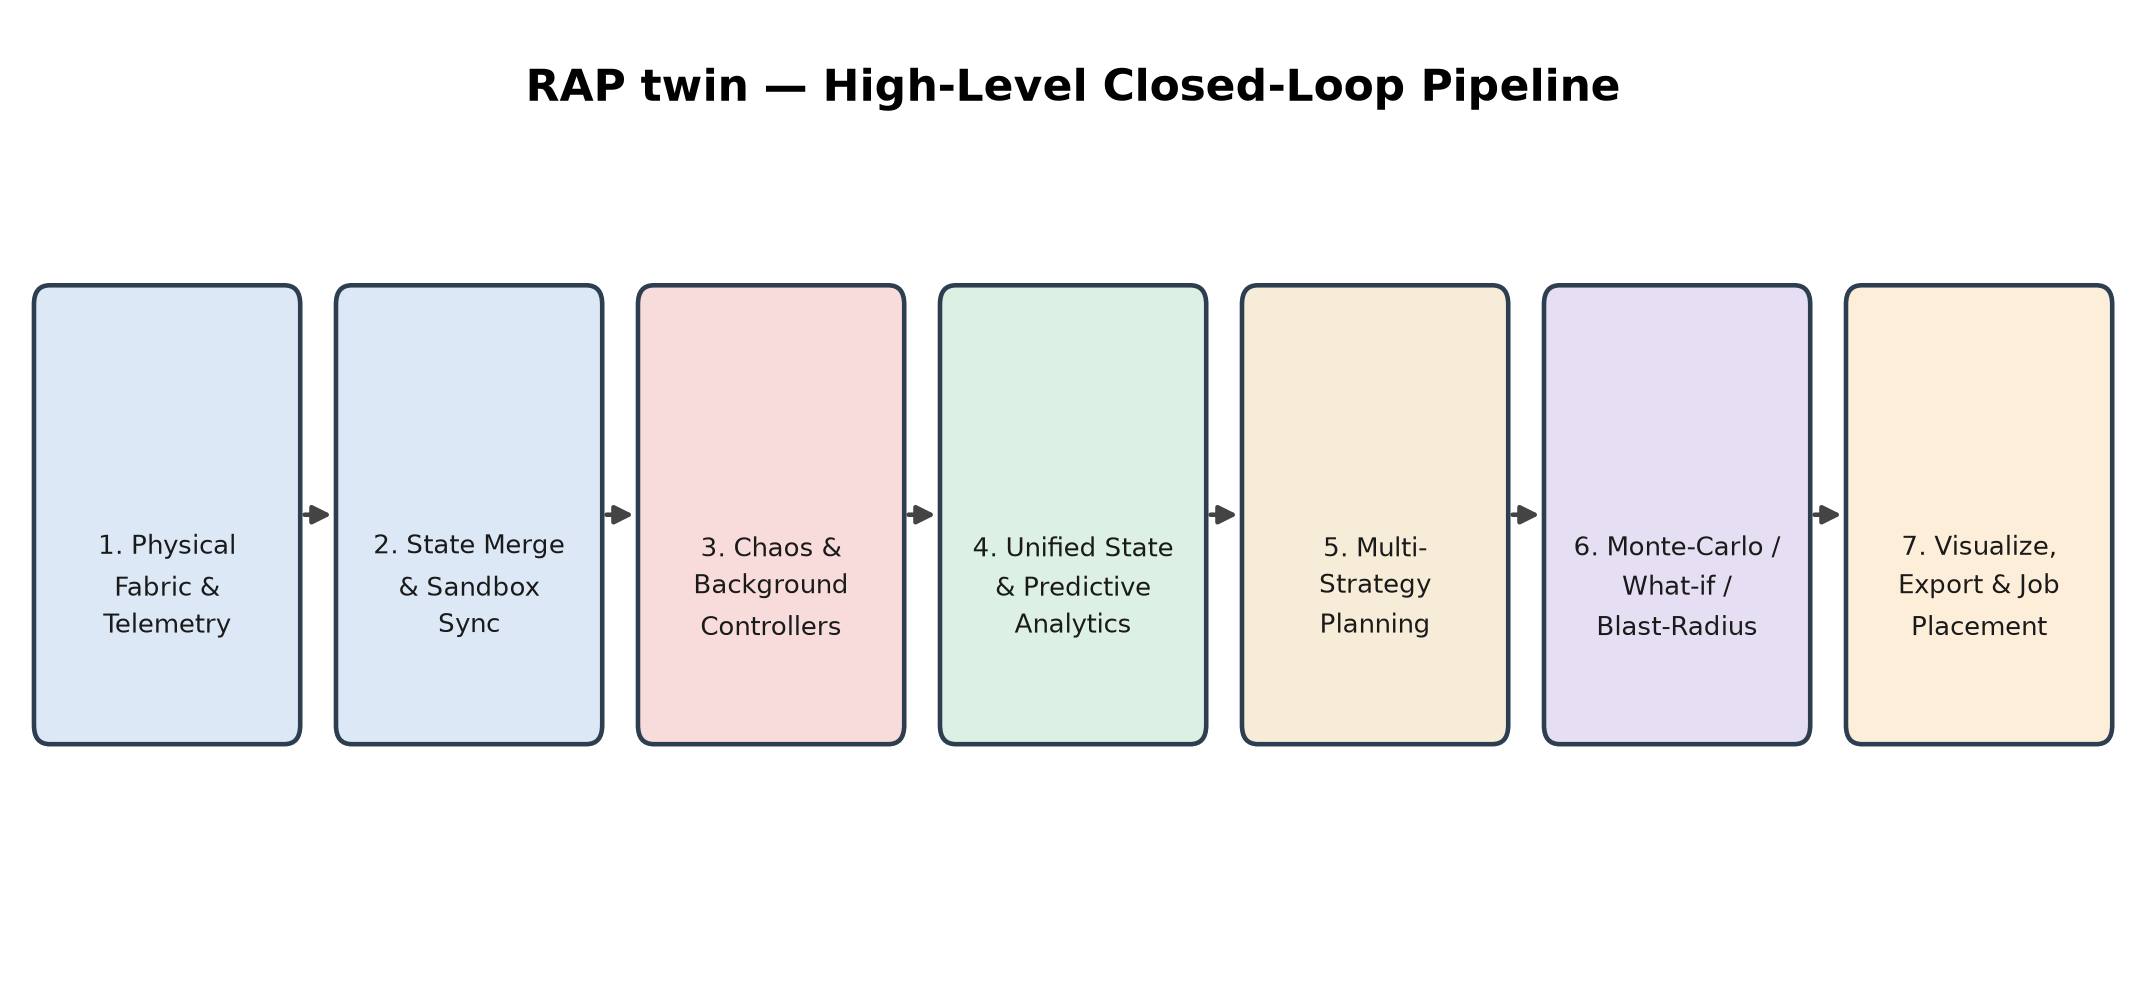
\includegraphics[width=\linewidth]{figures/pipeline_overview.png}
\caption{RAP twin -- High-Level Closed-Loop Pipeline}
\label{fig:pipeline-overview}
\end{figure}

The simulation and planning sub-pipeline (Fig.~\ref{fig:pipeline-simulation}) ensures high-fidelity, closed-loop emulation from raw telemetry ingestion to statistical performance evaluation:

\begin{enumerate}
    \item \textbf{State Management \& Telemetry Ingestion:} static descriptors and job descriptors (SLAs, multi-stage workflows, resource hints) are parsed and standardized; live telemetry is continuously merged via \texttt{/observe}; background controllers clean up expired reservations and monitor node reliability.
    \item \textbf{Multi-Strategy Workload Planning:} the pluggable planning engine assigns workloads using the selected strategy; a dry-run evaluator predicts placement outcomes so users can safely perform ``what-if'' analysis without committing resources.
    \item \textbf{Chaos Engineering \& Fault Injection:} the Chaos Engine injects deterministic, physical-layer failures so scheduling policies can be observed adapting and rerouting under real-world unpredictability.
    \item \textbf{Cost/Carbon, What-If \& Blast-Radius Analysis:} every plan is priced in money and carbon; proposed capacity changes are evaluated on a forked twin; the smallest fault set that breaks a given job is found automatically.
    \item \textbf{Dashboard Preview, CI Gate \& Export:} users get a real-time visualization of topology, predictive health, and job history; the CI resilience gate can fail a build on regression; the final twin state can be exported to Azure DTDL or Kubernetes CRDs.
\end{enumerate}

\begin{figure}[H]
\centering
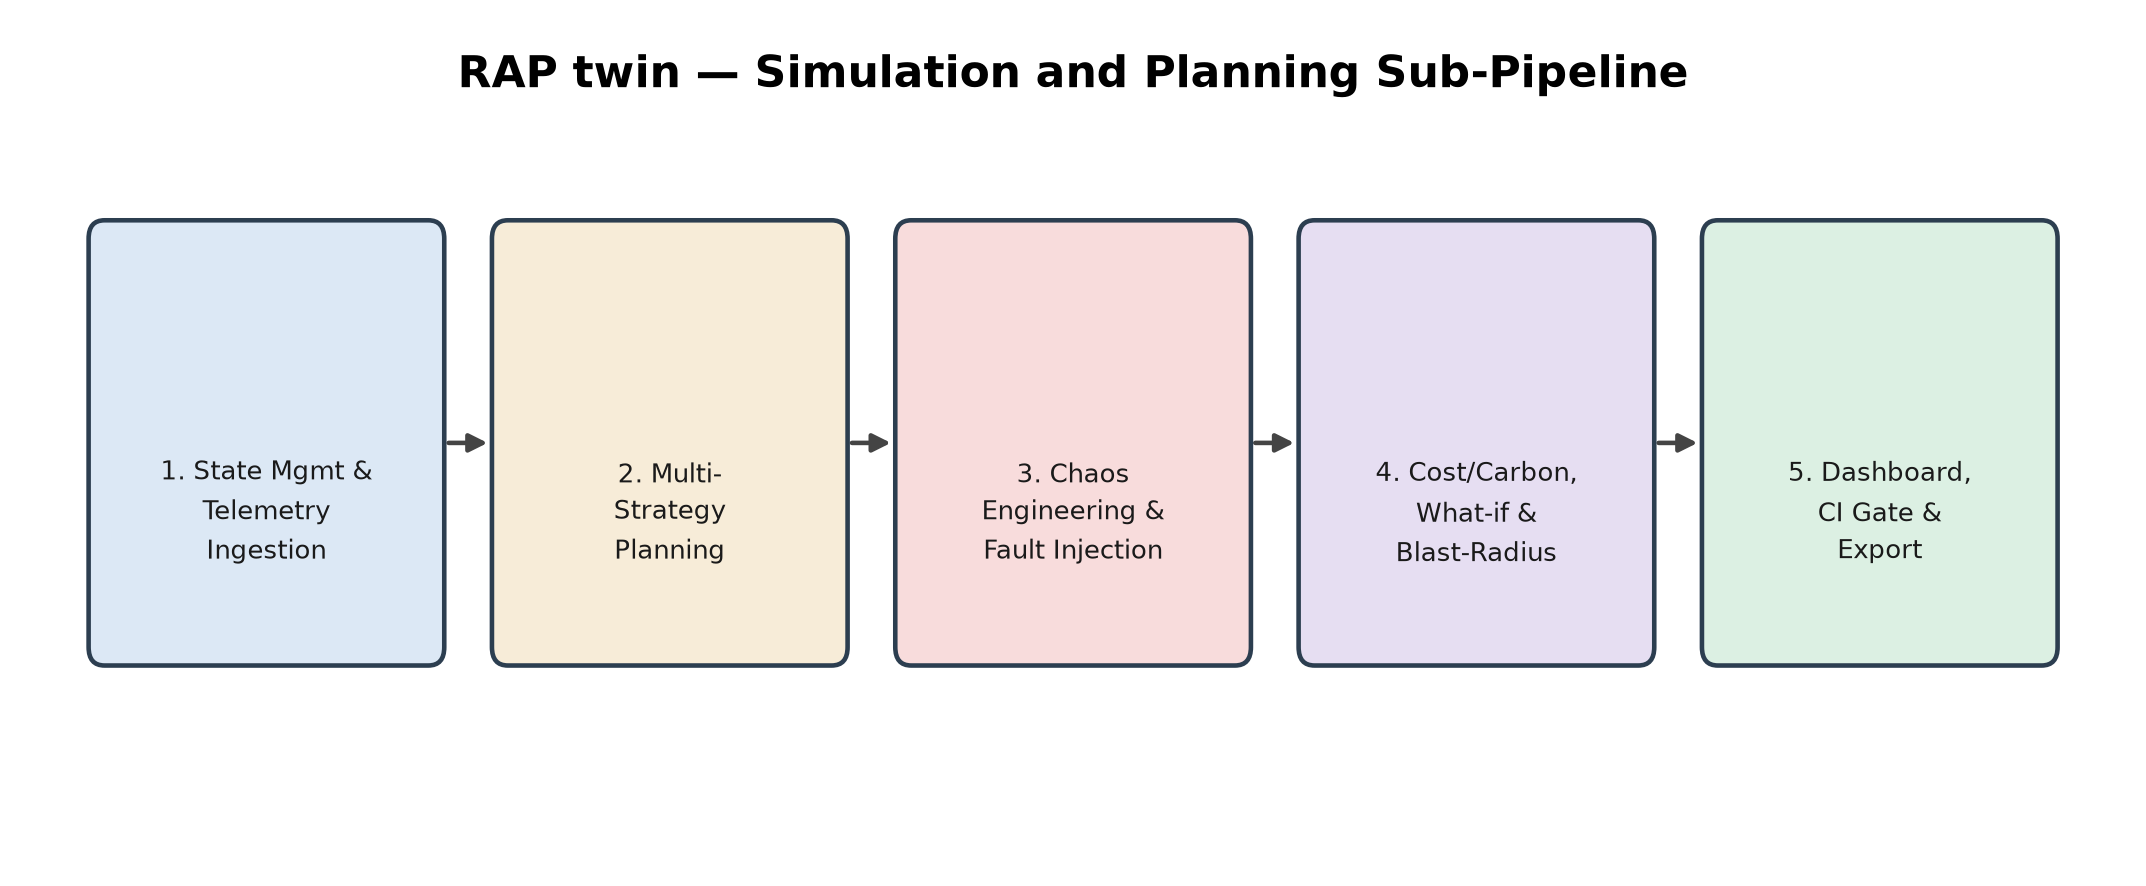
\includegraphics[width=\linewidth]{figures/pipeline_simulation.png}
\caption{RAP twin -- Simulation and Planning Sub-Pipeline}
\label{fig:pipeline-simulation}
\end{figure}

\section{Outcome}

The direct outcome of this project is a working, tested, and deployed platform: a Flask REST API exposing 25 endpoints, six pluggable scheduling strategies, a chaos engine wired into an automated CI resilience gate, cost/carbon accounting, blast-radius and what-if analysis tools, incident bundle export/import, a Kubernetes cluster importer, an MQTT telemetry sidecar, and a real-time React/TypeScript dashboard. The platform is covered by 129 automated tests and has been verified against a live deployment. Measured benchmarks (Chapter~\ref{chap:results}) show concrete, honestly-reported trade-offs between the available strategies rather than a single policy declared the winner on every metric.

\subsection{Type of Project}

RAP twin is primarily application-oriented, with a focus on practical implementation and real-world problem-solving within the domain of distributed computing fabrics and edge orchestration.

\textbf{Application-Oriented:} the core goal is a functional, deployable sandbox usable by researchers and engineers in Industry 4.0 smart manufacturing, 5G/6G telecommunications, and the Internet of Vehicles, to automate and optimize job placement, scheduling, and performance analytics. The platform is designed for immediate practical use, offering a dashboard, CLI, and REST API that safely simulate closed-loop edge emulation without risking live production infrastructure.

\textbf{Domain-Specific:}
\begin{itemize}
    \item \textit{Edge Computing \& 5G/6G Networks:} RAP twin safely manages and orchestrates heterogeneous workloads, addressing siloed telemetry, resource constraints, and time-sensitive task offloading.
    \item \textit{Chaos Engineering \& CI:} deterministic fault injection, Monte-Carlo tooling, and a CI resilience gate validate policy resilience and SLA hit rates under simulated real-world uncertainty.
    \item \textit{Artificial Intelligence:} RAP twin harnesses Multi-Agent Deep Reinforcement Learning, federated learning, and Markov Decision Processes to automate resource allocation and transform raw telemetry into actionable predictive insights.
\end{itemize}

\textbf{Research-Oriented:} the project also incorporates research elements in translating theoretical AI models into a practical engineering environment -- particularly in handling the ``estimation deviation'' between a digital twin's virtual predictions and actual physical hardware states, and in honestly characterizing where a sophisticated policy (RL-Markov) under-performs a simpler one on a non-latency metric (cost), which is itself a research-relevant finding reported in Chapter~\ref{chap:results} rather than concealed.



\chapter{PROJECT PLAN}

\section{Project Timeline}
    \createGanttChart
 
\section{Team Organization}

The project is carried out by a group of three team members, each assigned a specific role to ensure effective collaboration and clear reporting mechanisms.

\subsection{Team Structure}
\label{sec:team-structure-anchor}

\textbf{1. Riaan -- Digital Twin API \& Platform Infrastructure.} Responsible for the core digital twin infrastructure, state management, and platform-level concerns that every other module depends on.

\begin{itemize}
    \item Digital Twin API (Flask) backend development across all 25 REST endpoints.
    \item Unified State Machine (\texttt{dt.state.DTState}) implementation and hot-reloading.
    \item Live telemetry ingestion (\texttt{/observe} endpoint) and the MQTT telemetry sidecar.
    \item Background self-healing controllers (\texttt{SelfHealingController} \& \texttt{ResourceGuardian}).
    \item REST API security (\texttt{FABRIC\_API\_KEY} auth on mutating routes) and interoperability exporters (DTDL, Kubernetes CRDs) and importer.
    \item Incident bundle export/import tooling and the real-time dashboard's data layer.
\end{itemize}

\textbf{2. Avanti -- Intelligent Planning \& AI Scheduling.} Responsible for the multi-strategy planning engine, workload constraint parsing, and the advanced AI scheduling policies.

\begin{itemize}
    \item Multi-strategy planning engine and the shared planner factory (\texttt{dt/planners.py}).
    \item Federated/Resilient planner and RL-Markov (MDP) policy implementation.
    \item Cost- and carbon-aware strategies (Cheapest-Cost, Greenest) built on \texttt{dt/economics.py}.
    \item Planner CLI development and the dry-run / batch-planning evaluator.
    \item Job descriptor parsing, SLA constraints, and schema validation (YAML/JSON).
    \item What-if capacity planning (\texttt{dt/whatif.py}).
\end{itemize}

\textbf{3. Preet -- Simulation, Chaos Engineering \& Analytics.} Responsible for rigorously evaluating the system under real-world uncertainty, large-scale benchmarking, and resilience validation.

\begin{itemize}
    \item Chaos engine development (deterministic fault and noise injection).
    \item Chaos-as-CI resilience gate (\texttt{tools/ci\_gate.py}) and baseline regression checks.
    \item Blast-radius finder (\texttt{sim/blast\_radius.py}) for minimal-fault-set search.
    \item Monte Carlo simulation tooling and orchestration.
    \item Predictive analytics and failure forecasting (\texttt{PredictiveAnalyzer}).
    \item Statistical policy evaluation and benchmark reporting (Section~\ref{sec:performance-parameters}).
\end{itemize}

\chapter{SOFTWARE REQUIREMENT \vspace*{0.5\baselineskip} SPECIFICATION}
This chapter summarizes the requirements captured in full detail in the project's standalone Software Requirements Specification document (\texttt{RAPtwin\_SRS\_v1.2.docx}), which enumerates 31 individually status-tagged functional requirements (FR-01 through FR-31, each marked Implemented, In Progress, or Planned) and a complete set of use-case reports.

\section{Functional Requirements}

\begin{itemize}
    \item \textbf{State and telemetry:} parse and hot-reload static YAML descriptors; merge streaming telemetry via \texttt{/observe} or the MQTT sidecar; validate all payloads against JSON Schema; track per-node/link estimation deviation ($\Delta f$).
    \item \textbf{Predictive analytics:} forecast per-node utilization, thermal derating risk, and wireless link-loss variability.
    \item \textbf{Planning:} route DAG jobs through a pluggable interface supporting six strategies (Greedy, Cheapest-Energy, Cheapest-Cost, Greenest, Resilient/Federated, RL-Markov), with dry-run and batch-planning modes.
    \item \textbf{Chaos and self-healing:} inject deterministic chaos scenarios (link outages, packet noise, thermal throttling); start/stop chaos via REST; automatically reroute degraded jobs and reclaim expired reservations.
    \item \textbf{Economics:} compute cost (INR) and carbon (CO\textsubscript{2}) for every plan via \texttt{dt/economics.py}.
    \item \textbf{Resilience tooling:} run large-scale Monte-Carlo sweeps; evaluate what-if capacity changes without mutating the live twin; find the minimal fault set that breaks a job (blast-radius); gate CI builds on resilience regression.
    \item \textbf{Interoperability:} export twin state to Azure DTDL and Kubernetes CRDs; import a live Kubernetes cluster as a twin; export/import reproducible incident bundles.
    \item \textbf{Presentation:} serve a real-time web dashboard (topology, node health, job history, cost/carbon, chaos and what-if panels) over Server-Sent Events.
\end{itemize}

Three requirements remain Planned per the SRS's own status tagging as of this report's most recent SRS revision, two of which have since been implemented in the current codebase and should be re-verified against the live SRS document before final submission: GPU device requests in the containerized fabric launcher, MQTT telemetry ingestion, and REST API authentication -- all three now exist in the codebase (\texttt{fabric\_docker/launch\_fabric.py}, \texttt{sim/mqtt\_bridge.py}, \texttt{FABRIC\_API\_KEY}), so the SRS's status column is stale and should be refreshed to Implemented.

\section{Non-Functional Requirements}

\begin{itemize}
    \item \textbf{Performance:} baseline heuristic planners return a placement decision in under 5\,ms; a 1,000-trial Monte-Carlo sweep completes within a practical local benchmarking session.
    \item \textbf{Reliability:} the self-healing controller reroutes an affected job before its SLA deadline where a fallback exists; a single failed Monte-Carlo trial does not abort the sweep.
    \item \textbf{Security:} mutating REST routes require an \texttt{X-API-Key} header matching \texttt{FABRIC\_API\_KEY}; all input payloads are validated against JSON Schema before being merged into state.
    \item \textbf{Observability:} state changes are published as CloudEvents-formatted notifications on an internal event bus and streamed to the dashboard over Server-Sent Events (\texttt{/stream}, \texttt{/events}).
    \item \textbf{Maintainability:} new scheduling strategies can be added by implementing the pluggable planner interface under \texttt{dt/policy/} without touching the core state engine or API layer.
\end{itemize}

\section{Constraints}
\label{sec:constraints-design}

\begin{itemize}
    \item RAP twin runs as a single local process/workstation; it simulates a distributed fabric but is not itself horizontally distributed.
    \item The file-watcher hot-reload introduces a bounded latency ($\sim$0.5\,s) between an on-disk descriptor change and the state engine picking it up.
    \item Persistent state is file-based (YAML/JSON descriptors and an in-memory state object); there is no relational database.
    \item The Flask development server is not configured for high-availability, multi-instance horizontal scaling out of the box.
\end{itemize}

\section{Hardware Requirements}

\textbf{Client side:} any workstation, tablet, or phone with a modern web browser (Chrome, Firefox, Edge) and network access to the server.

\textbf{Server side:} a standard x86\_64 workstation or server with at least 4 CPU cores and 4\,GB RAM. Development and benchmarking were carried out on an Intel i7-13700K CPU with an NVIDIA RTX 4090 GPU (24\,GB VRAM); the GPU is tracked as a schedulable resource for containerized launches and is not required for the core simulation, chaos, or dashboard functionality, which is CPU-bound.

\section{Software Requirements}

\begin{itemize}
    \item Python 3.12, Flask (\texttt{>=3.0}), PyYAML, jsonschema, NumPy, Pandas, Matplotlib, rich.
    \item pytest, black, isort, ruff for testing and code quality (129 passing tests).
    \item React 19, TypeScript, Vite, TailwindCSS 4, D3.js, TanStack Query (dashboard frontend).
    \item Docker (optional, for the containerized fabric launcher) and an MQTT broker (optional, for the telemetry sidecar, via \texttt{requirements-mqtt.txt}).
    \item Git for version control.
\end{itemize}

\section{Interfaces}

RAP twin exposes 25 REST endpoints grouped by function: \textit{state and telemetry} (\texttt{/health}, \texttt{/snapshot}, \texttt{/observe}, \texttt{/topology}, \texttt{/nodes/<name>}); \textit{planning} (\texttt{/plan}, \texttt{/plan\_batch}, \texttt{/plans}, \texttt{/jobs}, \texttt{/release}); \textit{chaos and resilience} (\texttt{/chaos}, \texttt{/chaos/start}, \texttt{/chaos/stop}, \texttt{/whatif}, \texttt{/blast\_radius}, \texttt{/overrides/reset}); \textit{economics} (\texttt{/economics}); \textit{topology editing} (\texttt{/add\_node}, \texttt{/links}); \textit{interoperability} (\texttt{/standards/dtdl}, \texttt{/standards/crds}, \texttt{/bundle}); and \textit{live updates} (\texttt{/stream}, \texttt{/events}). All requests and responses use JSON except file-based bundle import/export. The frontend communicates with the backend exclusively over this REST surface and Server-Sent Events.

\chapter{DETAILED DESIGN}
\label{chap:detailed-design}

\section{Architectural Design}

Fig.~\ref{fig:architecture-current} shows the current architecture. Static descriptors and streaming telemetry are unified by the State Engine (\texttt{dt.state.DTState}), which exposes a state-query interface to the Predictive Analytics engine and the Planner Factory (six pluggable strategies). The Chaos \& Guardrails layer and the Economics module sit alongside the planner, injecting faults and pricing every plan respectively. Below them, four tool layers -- Analysis Tools (Monte-Carlo, what-if, blast-radius), the CI Resilience Gate, the Interoperability layer (DTDL/CRD export, cluster import), and Incident Bundles -- consume and produce twin state without ever mutating the live fabric outside of an explicit plan commit. An MQTT sidecar and the authenticated REST API form the ingestion/egress boundary, and the React dashboard is the primary human interface, closing the loop back to an external control plane or the physical/simulated fabric itself.

\lofsection{System Architecture}
\begin{figure}[H]
\centering
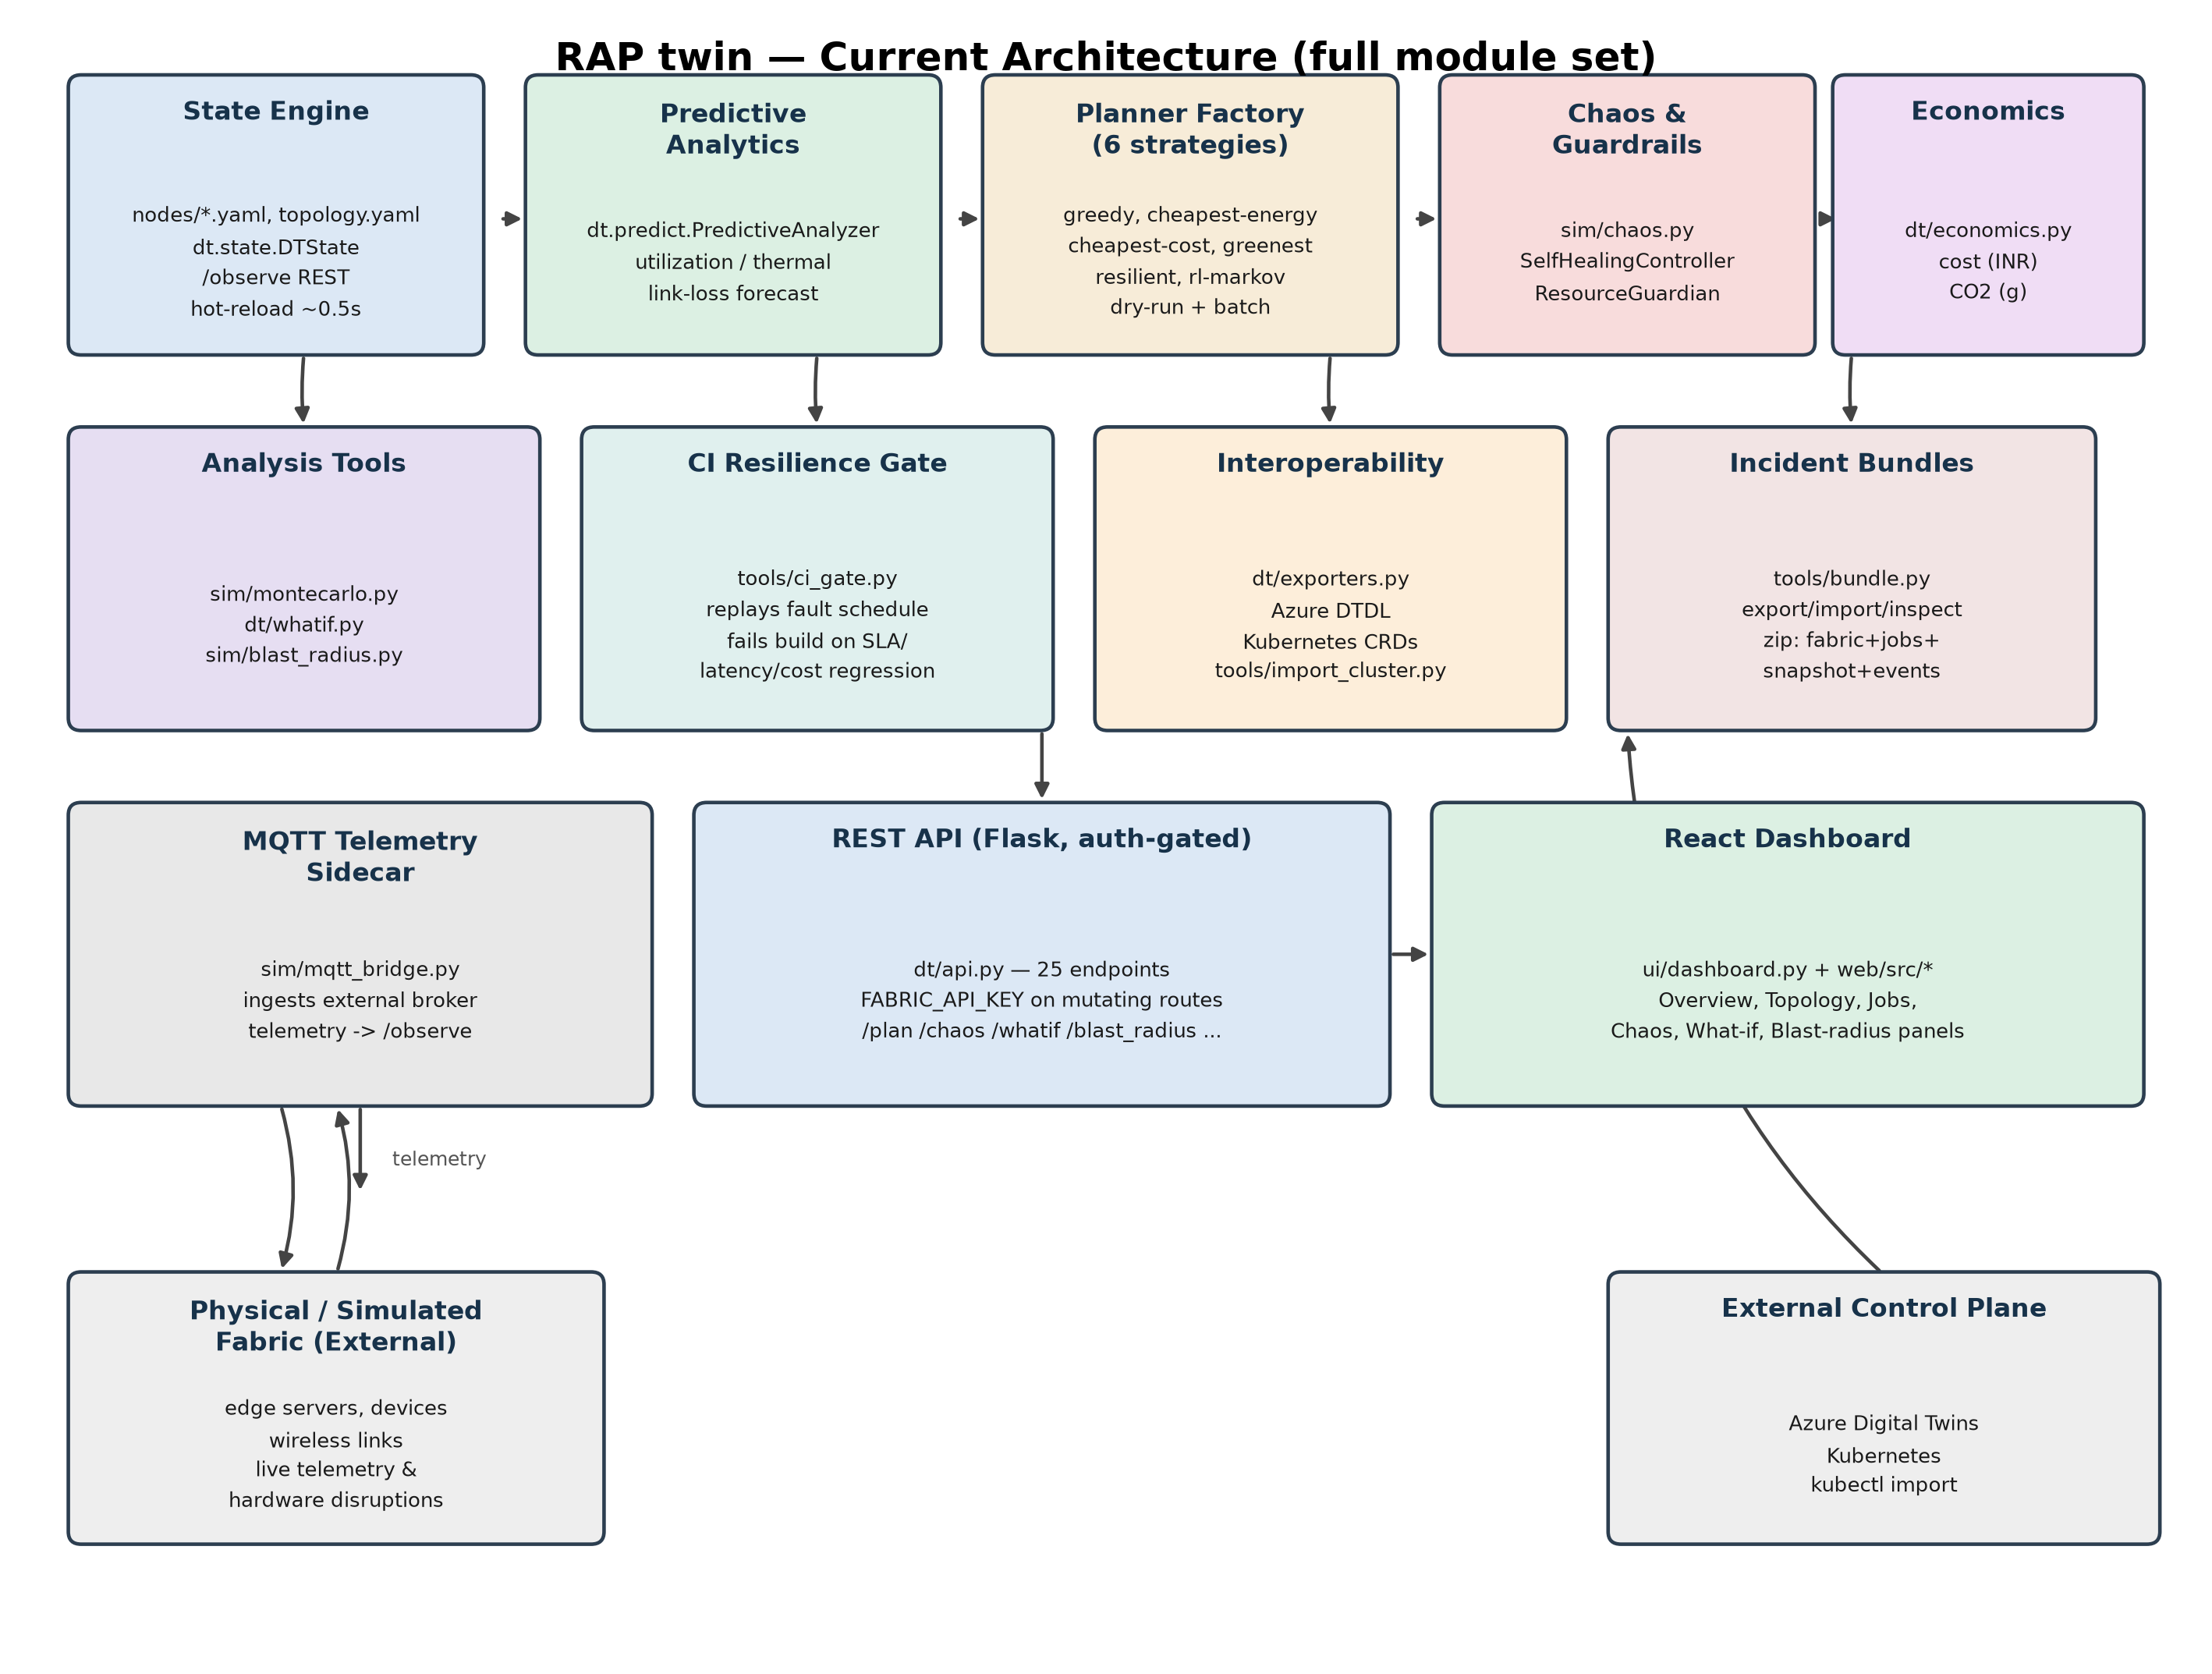
\includegraphics[width=\linewidth]{figures/architecture_current.png}
\caption{RAP twin -- Current Architecture (full module set)}
\label{fig:architecture-current}
\end{figure}

\section{Overview of Project Modules}
\label{sec:project-modules}

\begin{itemize}
    \item \textbf{State Engine} (\texttt{dt/state.py}, \texttt{dt/validators.py}): the central \texttt{DTState} class; merges static YAML descriptors with streaming telemetry; hot-reloads on-disk changes every $\sim$0.5\,s; validates all inputs against JSON Schema.
    \item \textbf{Predictive Analytics} (\texttt{dt/predict.py}): the \texttt{PredictiveAnalyzer} forecasts per-node utilization, thermal derating, and link-loss variability, with checkpoint/restore support so that a what-if or blast-radius search does not permanently bias live forecasts.
    \item \textbf{Planner Factory} (\texttt{dt/planners.py}, \texttt{dt/policy/*.py}): a single factory with an alias table dispatches to one of six strategies -- Greedy, Cheapest-Energy, Cheapest-Cost, Greenest, Resilient/Federated, and RL-Markov (MDP) -- so the API, the CI gate, and the blast-radius search all describe the same planner identically.
    \item \textbf{Economics} (\texttt{dt/economics.py}): converts a plan into a bill -- compute rental, electricity, and egress cost in INR, and CO\textsubscript{2} in grams, using per-zone pricing and grid-carbon-intensity defaults from \texttt{topology.yaml}.
    \item \textbf{Chaos Engine \& Guardrails} (\texttt{sim/chaos.py}, \texttt{dt/chaos\_runner.py}, \texttt{dt/self\_heal.py}): deterministic, time-compressed fault injection (link outages, packet noise, thermal throttling, power surges); \texttt{SelfHealingController} reroutes degraded job reservations; \texttt{ResourceGuardian} reclaims expired ones.
    \item \textbf{CI Resilience Gate} (\texttt{tools/ci\_gate.py}): replays a fault schedule against the twin, plans the job catalogue at each point on the timeline, and fails the build if worst-case SLA, p95 latency, cost, or carbon breaches a threshold or regresses against a committed baseline; wired into \texttt{.github/workflows/resilience-gate.yml}.
    \item \textbf{Blast-Radius Finder} (\texttt{sim/blast\_radius.py}): a breadth-first search over fault-set size that finds the smallest, minimal set of faults that breaks a given job, and reports the single most-implicated fault.
    \item \textbf{What-If Planner} (\texttt{dt/whatif.py}): forks the twin, applies a proposed change (clone/add/remove/patch nodes, add/remove links), replays the job catalogue through both forks, and diffs SLA, p95 latency, cost, and CO\textsubscript{2}.
    \item \textbf{Monte-Carlo Orchestrator} (\texttt{sim/montecarlo.py}): generates synthetic workload profiles and executes automated trial sweeps under active chaotic conditions, aggregating mean/p95/p99 JCT, energy, and SLA hit rate into CSV/JSON reports.
    \item \textbf{Interoperability} (\texttt{dt/exporters.py}, \texttt{tools/import\_cluster.py}): serializes twin state to Azure DTDL and Kubernetes CRDs; conversely, imports a live Kubernetes cluster (via \texttt{kubectl get nodes -o json}) as a twin, mapping capacity, architecture, zone, GPU resources, and readiness.
    \item \textbf{Incident Bundles} (\texttt{tools/bundle.py}): exports one zip reproducing a run -- fabric, job catalogue, active faults, snapshot, events, and plans -- with the commit recorded in the manifest, so a bug report is replayable.
    \item \textbf{MQTT Telemetry Sidecar} (\texttt{sim/mqtt\_bridge.py}): an optional bridge that ingests telemetry from an external MQTT broker and forwards it into \texttt{/observe}, for deployments where telemetry is already on a message bus.
    \item \textbf{REST API} (\texttt{dt/api.py}, \texttt{ui/dashboard.py}): 25 Flask endpoints; mutating routes require an \texttt{X-API-Key} header matching \texttt{FABRIC\_API\_KEY}.
    \item \textbf{React Dashboard} (\texttt{web/src/*}): a real-time single-page application (Overview, TopologyGraph, NodesTable, LinksTable, JobComposer, ObservationPanel, FederationsPanel, EventsFeed, RecentPlans, PlanStages) rendering topology, node health, job history, cost/carbon, chaos status, and what-if/blast-radius results.
\end{itemize}

\section{User Interface}

The dashboard is a single-page React application served independently of the Flask API and communicating with it over REST and Server-Sent Events. It is organized into tabs, each backed by one or more of the components listed in Section~\ref{sec:project-modules}. Figures are grouped below by tab, matching the component that renders it; screenshots are captured from a running instance (\texttt{./run.sh}) or the live deployment and inserted at each marked point before final submission.

\lofsection{User Interface Screens}

\lofsubsection{Overview Screen}
Fabric-wide KPIs: node/link counts, aggregate utilization, and the most recent plan's cost and CO\textsubscript{2} (\texttt{Overview.tsx}).
% \begin{figure}[H]
% \centering
% \includegraphics[width=0.9\linewidth]{figures/ui_overview.png}
% \caption{Dashboard -- Overview tab}
% \label{fig:ui-overview}
% \end{figure}

\lofsubsection{Topology and Federations Screens}
An interactive, explorable graph of nodes and links (\texttt{TopologyGraph.tsx}), colour-coded by health and highlighting federation boundaries (\texttt{FederationsPanel.tsx}).
% \begin{figure}[H]
% \centering
% \includegraphics[width=0.9\linewidth]{figures/ui_topology.png}
% \caption{Dashboard -- Topology tab}
% \label{fig:ui-topology}
% \end{figure}

\lofsubsection{Nodes and Links Screens}
Tabular views (\texttt{NodesTable.tsx}, \texttt{LinksTable.tsx}) of every descriptor field, editable where the REST API supports it.
% \begin{figure}[H]
% \centering
% \includegraphics[width=0.9\linewidth]{figures/ui_nodes.png}
% \caption{Dashboard -- Nodes tab}
% \label{fig:ui-nodes}
% \end{figure}

\lofsubsection{Job Composer Screen}
A form and raw-JSON editor (\texttt{JobComposer.tsx}) for submitting a DAG job, choosing a strategy, and toggling dry-run.
% \begin{figure}[H]
% \centering
% \includegraphics[width=0.9\linewidth]{figures/ui_job_composer.png}
% \caption{Dashboard -- Job Composer tab}
% \label{fig:ui-job-composer}
% \end{figure}

\lofsubsection{Chaos and Faults Screens}
Start/stop a chaos scenario, view current overrides (\texttt{ObservationPanel.tsx}), run a blast-radius search, and download an incident bundle.
% \begin{figure}[H]
% \centering
% \includegraphics[width=0.9\linewidth]{figures/ui_chaos.png}
% \caption{Dashboard -- Chaos \& Faults tab}
% \label{fig:ui-chaos}
% \end{figure}

\lofsubsection{What-If Screen}
Define a proposed change set and view the forked-twin diff (SLA/p95/cost/CO\textsubscript{2}).
% \begin{figure}[H]
% \centering
% \includegraphics[width=0.9\linewidth]{figures/ui_whatif.png}
% \caption{Dashboard -- What-if tab}
% \label{fig:ui-whatif}
% \end{figure}

\lofsubsection{Recent Plans and Events Screens}
A live history of planning decisions and CloudEvents-formatted state changes (\texttt{RecentPlans.tsx}, \texttt{EventsFeed.tsx}, \texttt{PlanStages.tsx}).
% \begin{figure}[H]
% \centering
% \includegraphics[width=0.9\linewidth]{figures/ui_recent_plans.png}
% \caption{Dashboard -- Recent Plans tab}
% \label{fig:ui-recent-plans}
% \end{figure}

\section{Data design}
\subsection{Data structure}

RAP twin does not use a relational or NoSQL database management system. Persistent configuration is stored as static YAML files, and runtime state lives in the in-memory \texttt{DTState} object together with a JSON telemetry-override file. The principal on-disk structures are:

\begin{itemize}
    \item \texttt{nodes/*.yaml} -- per-node hardware descriptors: name, CPU, RAM, VRAM, architecture flags, power-draw profile, zone.
    \item \texttt{sim/topology.yaml} -- network topology (node list, links with bandwidth/latency/loss, and \texttt{defaults.pricing} / \texttt{defaults.energy} used by the economics module).
    \item \texttt{schemas/job.schema.yaml} -- validates incoming DAG job submissions (stages, resource requirements, SLA deadline, priority).
    \item \texttt{sim/overrides.json} -- live telemetry deltas merged into \texttt{DTState} via \texttt{/observe} (node or link, target key, changes).
    \item \texttt{plans/*.json} -- recorded planning/trial output, including Monte-Carlo trial logs.
\end{itemize}

\subsection{Database Description}

There is deliberately no database server in this project: a Topology has many Nodes; a Node has many Links to other Nodes; a Node holds zero or more active Job Reservations; a Job DAG has many Stages, each bound to exactly one Node once planned; a Chaos Scenario has many Chaos Events, each targeting one Node or Link. These relationships are enforced in-memory by \texttt{DTState} and its validators rather than by foreign keys. This keeps the sandbox dependency-free and trivially portable, at the cost of not yet supporting multi-process or multi-host deployments of the simulator itself -- a trade-off made explicitly, not by omission (Section~\ref{sec:constraints-design}).

\section{UML Diagrams}

\lofsection{UML Diagrams}
\begin{figure}[H]
\centering
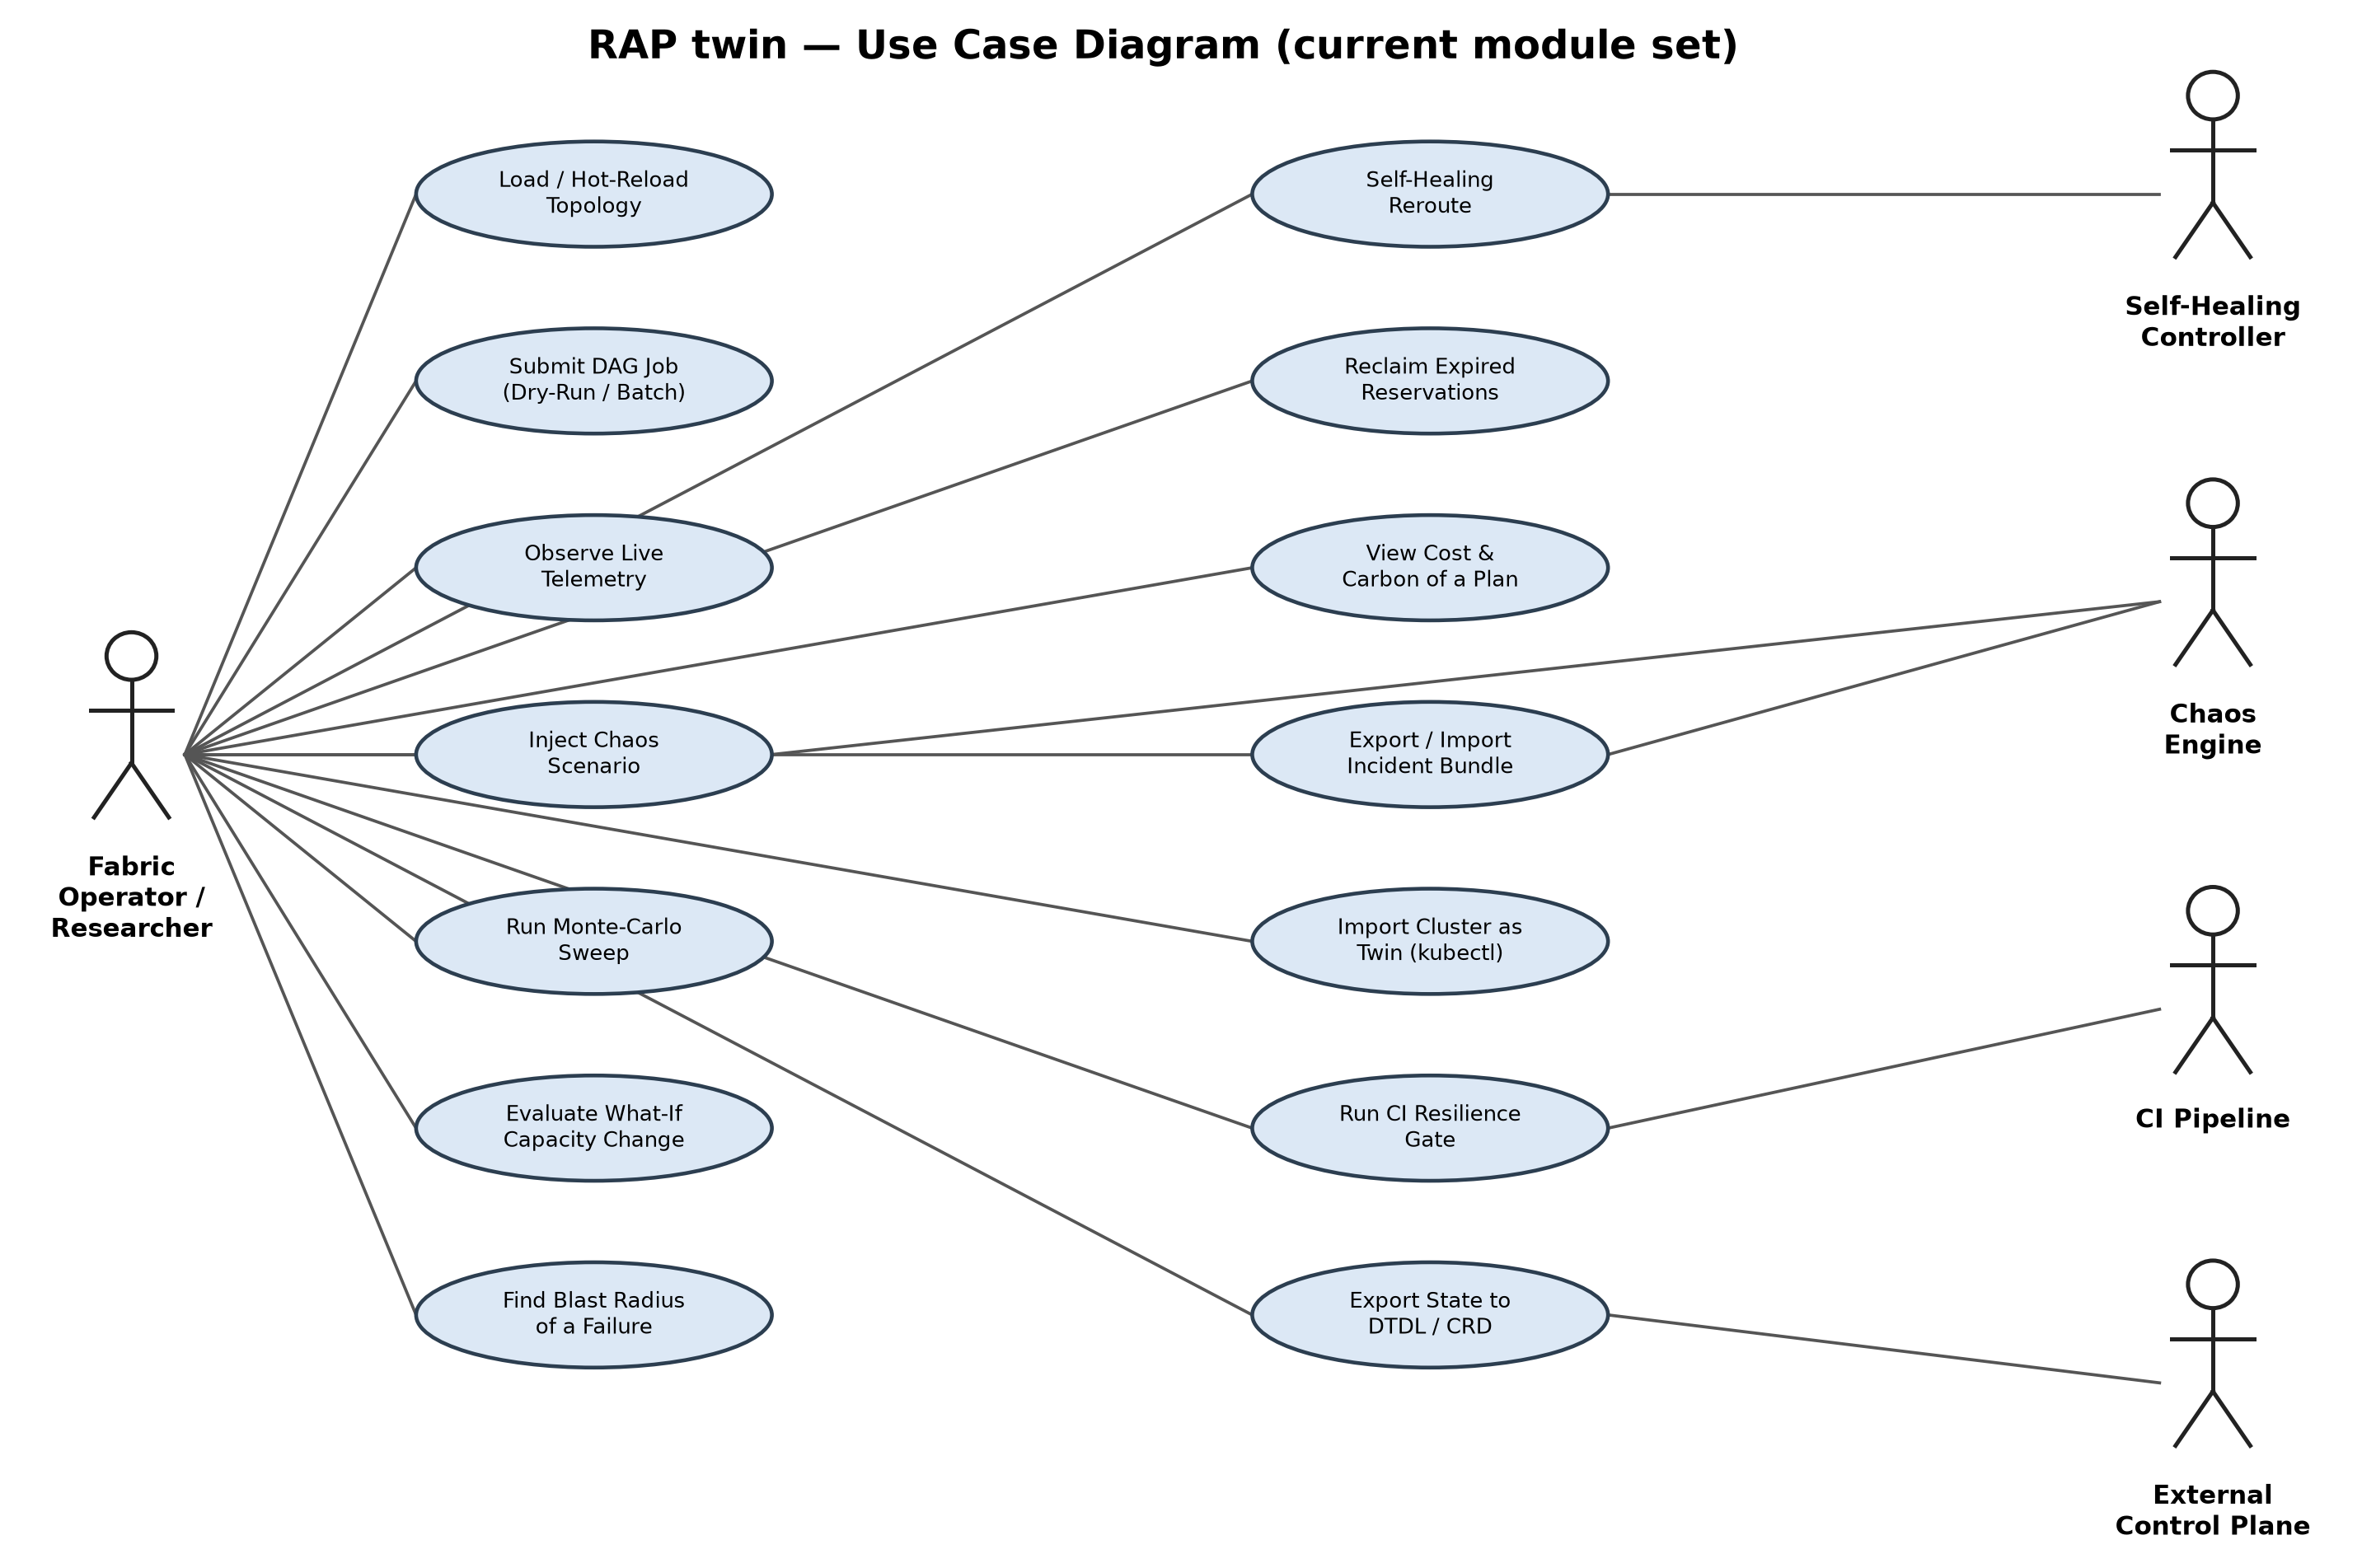
\includegraphics[width=0.95\linewidth]{figures/usecase_diagram.png}
\caption{Use Case Diagram}
\label{fig:usecase}
\end{figure}

\section{Tools and Technology Used}

Python 3.12 (Flask, PyYAML, jsonschema, NumPy, Pandas, Matplotlib, rich) for the backend; React 19, TypeScript, Vite, TailwindCSS 4, D3.js, and TanStack Query for the dashboard; pytest, black, isort, and ruff for testing and code quality; Docker (optional) for the containerized fabric launcher; an MQTT broker (optional) for the telemetry sidecar; Git/GitHub for version control and CI (GitHub Actions running the resilience gate on every relevant pull request).

\section{Algorithm}
\label{sec:algorithm}

This section details the \textbf{Resilient (Federated) planner}, chosen because its documented, measured trade-off (Section~\ref{sec:performance-parameters}) makes it the most instructive strategy to walk through in full.

\subsection{Resilient (Federated) Planner for Fault-Tolerant Placement}

The Resilient planner is the scheduling strategy in \texttt{dt/policy/resilient.py} responsible for network-aware job placement under uncertainty. Unlike the baseline Greedy and Cheapest-Energy heuristics, which optimize a single objective (resource fit or cost) and commit to the single best-scoring node, the Resilient planner treats every placement decision as a bet against future node or link failure, and reserves a verified fallback alongside the primary choice so that a mid-flight failure can be absorbed by the \texttt{SelfHealingController} without re-planning from scratch.

\subsection{Operational Mechanism}

The Resilient planner scores each candidate node not only on raw resource fit, as the Greedy planner does, but on a composite of (a) immediate resource fit, (b) the node's current predictive reliability score from \texttt{PredictiveAnalyzer}, and (c) the availability of at least one redundant fallback path to a secondary node in case the primary candidate degrades mid-flight. It therefore tends to prefer nodes that are not the single cheapest or fastest option, but that keep a viable fallback alive -- a property that only pays off once a fault actually occurs, which is exactly what the chaos-as-CI gate exists to measure.

\subsection{Algorithmic Workflow}

\begin{enumerate}
    \item For each stage of the submitted job DAG, enumerate candidate nodes that satisfy the stage's CPU/RAM/VRAM and architecture requirements.
    \item For each candidate, compute a composite score: resource-fit score $\times$ reliability score $\times$ fallback-availability bonus.
    \item Select the highest-scoring candidate as the primary placement; identify the next-highest-scoring candidate on a disjoint link path as the fallback.
    \item Reserve the primary placement (or, in dry-run mode, predict its outcome without reserving).
    \item If the \texttt{SelfHealingController} later detects the primary node degrading, reroute the in-flight stage to the pre-identified fallback.
    \item Repeat for every stage, respecting the DAG's dependency order.
\end{enumerate}

\subsection{Pseudocode}

\begin{algorithm}[H]
\SetAlgoLined
\KwIn{job DAG $J$, twin state $S$, predictive scores $R$}
\KwOut{placement plan $P$ with primary and fallback assignments}
$P \leftarrow \emptyset$\;
\ForEach{stage $s \in J.\text{stages (dependency order)}$}{
    $C \leftarrow \{n \in S.\text{nodes} : \text{fits}(s, n)\}$\;
    \ForEach{$n \in C$}{
        $\text{score}(n) \leftarrow \text{fit}(s, n) \times R[n] \times \text{fallback\_bonus}(n, C)$\;
    }
    $n^{*} \leftarrow \arg\max_{n \in C} \text{score}(n)$\;
    $n^{\text{fb}} \leftarrow \arg\max_{n \in C \setminus \{n^{*}\}, \text{disjoint\_path}(n, n^{*})} \text{score}(n)$\;
    $P \leftarrow P \cup \{(s, n^{*}, n^{\text{fb}})\}$\;
    \If{\textbf{not} dry\_run}{
        reserve($n^{*}$, $s$)\;
    }
}
\Return{$P$}\;
\caption{Resilient (Federated) Planner -- Stage Placement with Fallback}
\end{algorithm}

 \chapter{RESULTS AND DISCUSSION}
 \label{chap:results}
 \section{Experimental Setup}
 \subsection{Dataset}

Benchmarks were run against the project's own fabric and job catalogue (\texttt{nodes/}, \texttt{jobs/jobs\_10.yaml}, limited to the first 6 jobs for both tools so they see the same catalogue slice) rather than a synthetic literature-style scenario. Two measurement tools combine to produce the results below: \texttt{tools/policy\_benchmark.py} measures mean JCT and energy under normal operation (no chaos), and \texttt{tools/ci\_gate.py} measures p95 JCT and SLA hit rate under the \texttt{core\_link\_cut} chaos scenario at \texttt{deadline\_scale=0.28} (a margin-test setting established in \texttt{ci/gate.yaml}). These are two different operating conditions, not one unified run -- the benchmark's own output JSON (\texttt{reports/srs\_benchmark\_table.json}) states this explicitly, and that caveat is preserved here rather than smoothed over.

\lofsection{Datasets}
\begin{figure}[H]
\centering
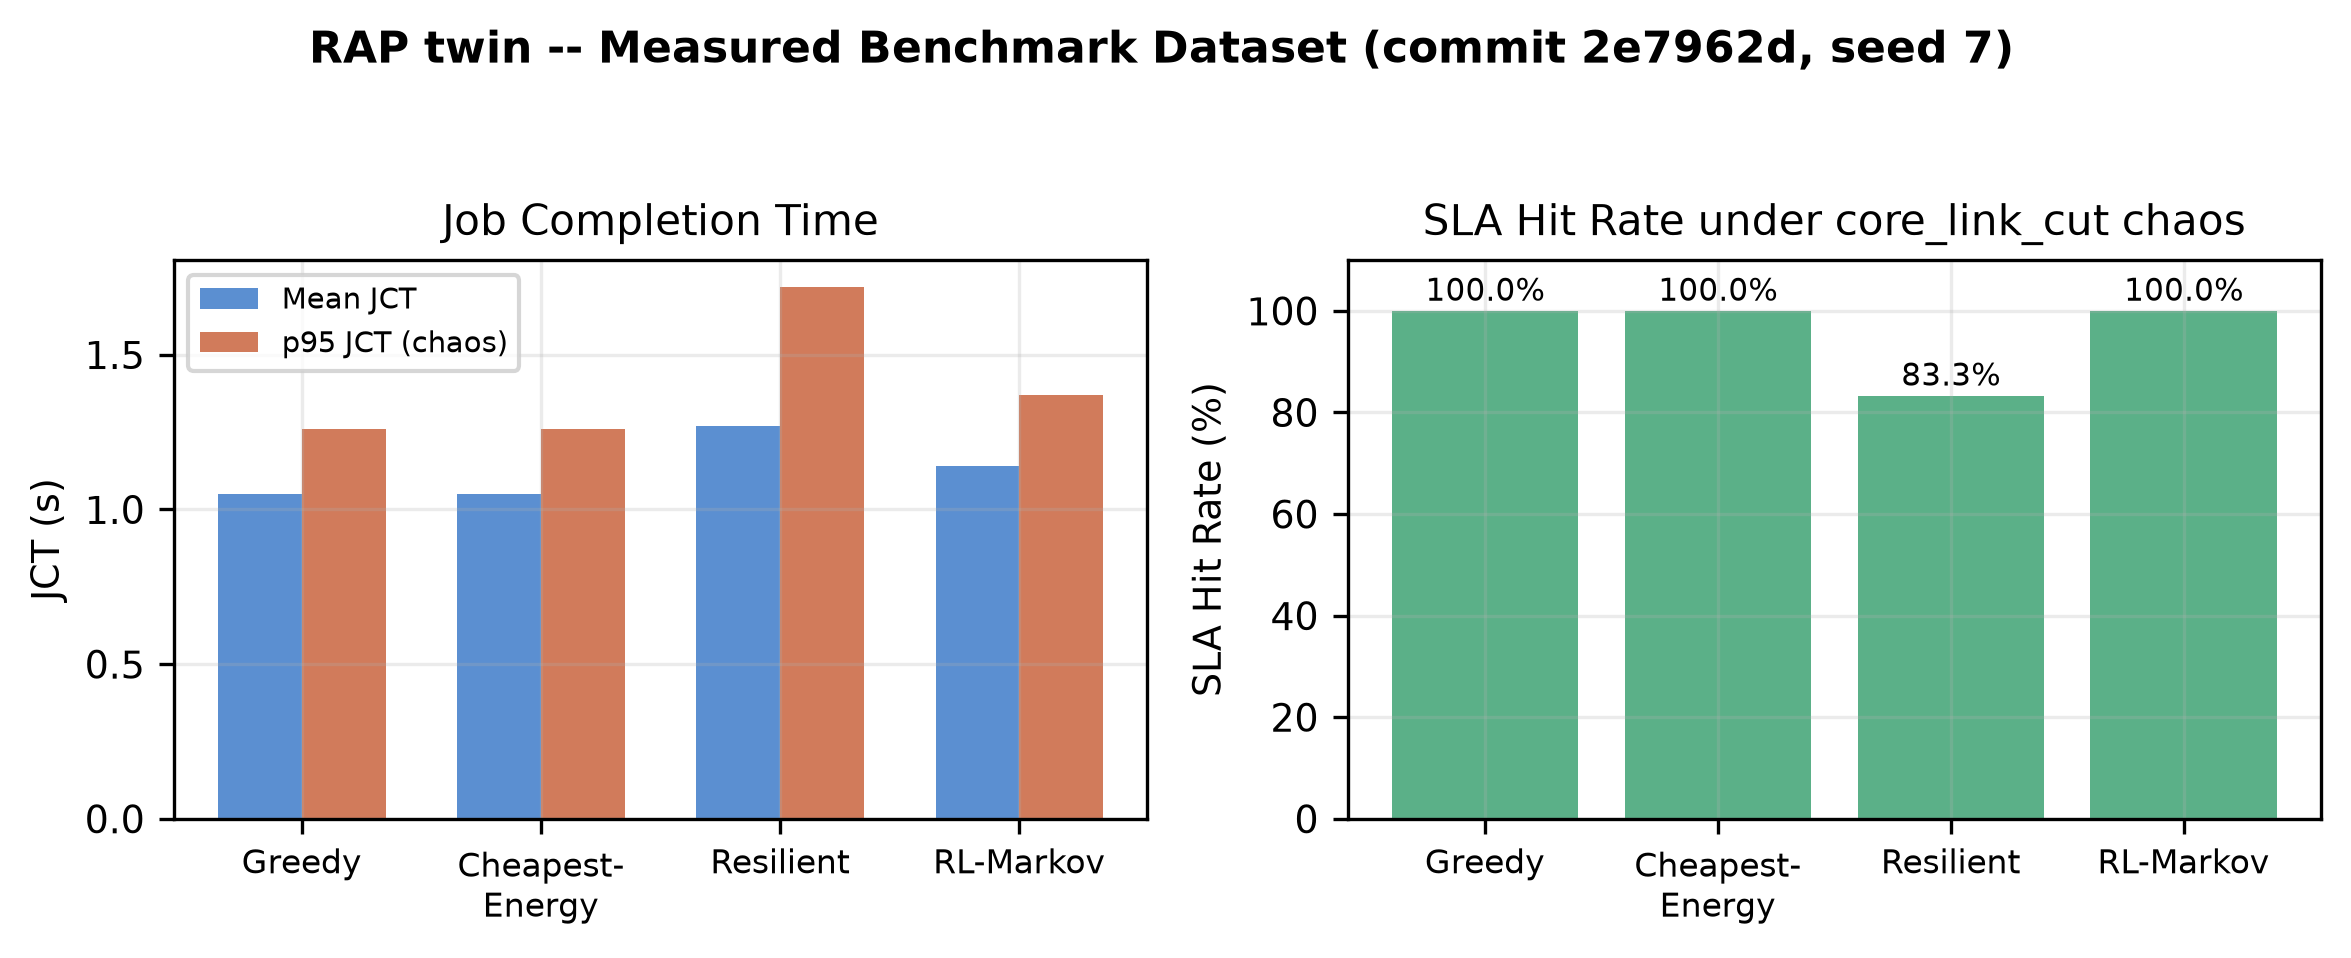
\includegraphics[width=0.95\linewidth]{figures/dataset_benchmark.png}
\caption{RAP twin -- Measured Benchmark Dataset (commit \texttt{2e7962d}, seed 7)}
\label{fig:dataset-benchmark}
\end{figure}

\subsection{Performance Parameters}
\label{sec:performance-parameters}

\begin{table}[H]
\centering
\caption{Measured Benchmark Table (commit \texttt{2e7962d}, seed 7, job\_limit 6)}
\label{tab:performance-parameters}
\begin{tabular}{|l|c|c|c|c|}
\hline
\textbf{Strategy} & \textbf{Mean JCT (s)} & \textbf{p95 JCT (s)} & \textbf{Energy (J)} & \textbf{SLA Hit Rate} \\
\hline
Greedy & 1.05 & 1.26 & 13.0 & 100.0\% \\
Cheapest-Energy & 1.05 & 1.26 & 13.0 & 100.0\% \\
Resilient & 1.27 & 1.72 & 13.0 & 83.3\% \\
RL-Markov & 1.14 & 1.37 & 16.2 & 100.0\% \\
\hline
\end{tabular}
\end{table}

\noindent\textit{Note: Mean JCT and Energy were measured under normal operation; p95 JCT and SLA Hit Rate were measured separately under the \texttt{core\_link\_cut} chaos scenario at \texttt{deadline\_scale=0.28}. These are two different operating conditions, not one unified experiment.}

\subsection{Efficiency Issues}

Three findings are reported here exactly as the engineering worklog recorded them, including the ones that are not flattering:

\begin{itemize}
    \item \textbf{The Resilient planner trades latency for fallback coverage, and under a tightened deadline it loses on SLA, not just speed.} Table~\ref{tab:performance-parameters} shows Resilient's p95 JCT (1.72\,s) is 36\% higher than Greedy's (1.26\,s), and at \texttt{deadline\_scale=0.28} its SLA hit rate (83.3\%) is lower than Greedy's (100\%). This is stated plainly rather than presenting Resilient as a strict improvement: it buys redundant fallback coverage, which this particular benchmark run does not end up needing enough to offset the latency cost.
    \item \textbf{An unresolved $\sim$75$\times$ cost anomaly in the RL-Markov planner.} Separately from the JCT/energy/SLA table above, the project's cost accounting (\texttt{dt/economics.py}) measured the RL-Markov planner costing approximately 75 times more than Greedy for the same job on the sample fabric (Rs.~0.894 vs.\ Rs.~0.012), because it spreads stages across sites and the cross-site egress bill dominates. This is recorded as an open question in \texttt{WORKLOG.md} -- whether it is a genuine defect in the MDP planner's network penalty, or intended behaviour -- and is carried into Future Work (Section~\ref{sec:future-work}) rather than resolved here.
    \item \textbf{A predictive-state-leak bug, found and fixed during blast-radius development.} \texttt{PredictiveAnalyzer} was found to retain an elevated \texttt{projected\_derate} after a thermal-derate fault was reverted, so every evaluation after a derate trial was measuring an already-degraded fabric. This was fixed by adding \texttt{PredictiveAnalyzer.checkpoint()/restore()}, which the blast-radius search now wraps around every trial. The underlying stickiness is still the intended behaviour for the live twin (a real fabric's reliability history should persist), but it means a chaos run permanently biases the twin's forecasts until the process restarts -- \texttt{POST /overrides/reset} clears active faults but not predictive history, which is itself listed as an open question in Future Work.
\end{itemize}

 \section{Software Testing}
  \subsection{Test Cases and Test Results}

\begin{table}[H]
\centering
\caption{Test Case Summary}
\label{tab:test-case-summary}
\begin{tabular}{|l|c|p{6.3cm}|}
\hline
\textbf{Test File} & \textbf{Count} & \textbf{Covers} \\
\hline
\texttt{test\_api.py} & 3 & Core REST endpoint smoke tests \\
\texttt{test\_api\_auth.py} & 7 & \texttt{FABRIC\_API\_KEY} gating on mutating routes \\
\texttt{test\_management.py} & 15 & Node/link/job management endpoints \\
\texttt{test\_economics.py} & 11 & Cost/carbon arithmetic, hand-calculated cases \\
\texttt{test\_ci\_gate.py} & 17 & Resilience gate determinism and baseline comparison \\
\texttt{test\_blast\_radius.py} & 13 & Minimality of reported fault sets \\
\texttt{test\_bundle.py} & 10 & Incident bundle export/import round-trip \\
\texttt{test\_import\_cluster.py} & 17 & Kubernetes capacity/label mapping fidelity \\
\texttt{test\_whatif.py} & 11 & Fork-and-diff correctness, dry-run vs.\ committed fidelity \\
\texttt{test\_launch\_fabric.py} & 7 & Containerized fabric launcher \\
\texttt{test\_mqtt\_bridge.py} & 11 & MQTT telemetry ingestion sidecar \\
\texttt{test\_benchmark\_srs\_table.py} & 7 & Benchmark table generation script \\
\hline
\textbf{Total} & \textbf{129} & \\
\hline
\end{tabular}
\end{table}

All 129 tests pass (\texttt{python -m pytest tests}). Beyond unit tests, the resilience gate itself is verified deterministically -- two runs of \texttt{tools/ci\_gate.py} against the same inputs produce byte-identical results -- and the platform has been verified end to end against a live deployment (every REST endpoint returning 200, a real plan returning real cost/CO\textsubscript{2}, what-if and blast-radius returning real reports).

 \section{Summary}
 \subsection{Result Analysis and Discussion}

The measured results in this chapter support three conclusions. First, there is no single scheduling strategy that wins on every metric: Resilient's redundancy costs latency and, in this configuration, SLA hit rate, which is a genuine trade-off rather than a defect. Second, RL-Markov's cost behaviour is not yet fully understood and is reported as an open question rather than quietly omitted. Third, the project's own tooling (checkpoint/restore, the CI resilience gate, 129 passing tests) is itself a result: it is what makes a trade-off like Resilient's measurable and reproducible in the first place, rather than anecdotal.

 \chapter{CONCLUSION AND \vspace*{0.5\baselineskip} FUTURE WORK}

 \section{Conclusions}

RAP twin delivers a working, tested, and deployed digital-twin planning sandbox: a unified state engine synchronizing static descriptors with live telemetry; six pluggable scheduling strategies with dry-run and batch modes; a deterministic chaos engine wired directly into an automated CI resilience gate; cost and carbon accounting for every plan; blast-radius and what-if analysis tools; a Kubernetes cluster importer and DTDL/CRD exporters; reproducible incident bundles; and a real-time React dashboard. All of this is covered by 129 automated tests and has been verified against a live deployment. Just as importantly, the project's benchmarking methodology surfaces genuine trade-offs (Resilient's latency cost for fallback coverage) and open questions (the RL-Markov cost anomaly) rather than presenting only favourable numbers, which is itself a deliverable of an honestly-engineered resilience-testing platform.

 \section{Future Work}
 \label{sec:future-work}

Four concrete, specific items remain open, carried directly from the project's own engineering worklog rather than invented for this report:

\begin{enumerate}
    \item \textbf{Investigate the RL-Markov cost anomaly.} Determine whether the $\sim$75$\times$ cost penalty relative to Greedy (Section~\ref{sec:performance-parameters}) is a genuine defect in the MDP planner's network-egress penalty, or intended behaviour that should instead be explained and documented for users.
    \item \textbf{Decide whether chaos recovery should rewind predictive history.} \texttt{POST /overrides/reset} currently clears active faults but not the \texttt{PredictiveAnalyzer}'s accumulated history, so a fabric that has run chaos plans differently until the process restarts. Whether this stickiness should be optional needs a decision.
    \item \textbf{Add a deliberately tight catalogue or smaller fabric for demonstration.} The sample fabric is roughly 3--4$\times$ over-provisioned for the sample job catalogue, which masks several features' effects out of the box; a tighter sample configuration would make trade-offs like Resilient's visible without needing \texttt{deadline\_scale} tuning.
    \item \textbf{Respect declared link profiles on load.} Link profiles (e.g.\ \texttt{IB-400G}) are currently ignored on load and plan as a default 10\,Gbps / 1\,ms link, which makes every latency number for a profile-only link wrong. This is flagged in the project's own worklog as the highest-value correctness fix outstanding, since fixing it will change planner results and requires a re-baseline of the CI gate.
\end{enumerate}

 \section{Application}

RAP twin is directly applicable to: \textit{pre-production capacity planning} (using the what-if planner to answer "would two more nodes fix our deadline misses?" before purchasing hardware); \textit{resilience and chaos testing} (using the chaos-as-CI gate to catch a scheduling regression before it reaches production, the way unit tests guard application code); \textit{cost- and carbon-aware scheduling} (using the Cheapest-Cost and Greenest strategies, and the economics module's per-plan billing, to make deployment decisions that account for money and emissions, not just latency); and \textit{incident reproduction and postmortems} (using incident bundles to capture and replay the exact fabric state, faults, and plans around a production issue).
 
\clearpage
\pagenumbering{gobble}
\pagestyle{empty}

\makeatletter
\renewcommand{\@chapapp}{Annexure}
\renewcommand{\thechapter}{\Alph{chapter}}
\makeatother

% Custom annexure chapter style
\makeatletter
\renewcommand{\@makechapterhead}[1]{%
  \vspace*{\fill}%
  \begin{center}
    {\Huge\bfseries Annexure \thechapter\\[1.5ex]#1}
  \end{center}
  \thispagestyle{chaptertitle}% disable headers/footers
  \vspace*{\fill}
  \clearpage
}
\makeatother

\begin{appendices}

\chapter{Program Outcome and Program Specific Outcome Mapping}

\section{Program Outcome (PO) Mapping}

\begin{longtable}{|p{0.6cm}|p{6.3cm}|p{1cm}|p{6.5cm}|}
\hline
\textbf{PO} & \textbf{Description} & \textbf{Level} & \textbf{Justification} \\
\hline
\endhead
PO1 & Engineering knowledge: apply mathematics, science, and engineering fundamentals to complex engineering problems. & 3 & RAP twin applies mathematical modelling (MDP, cost/carbon optimization) and distributed-systems engineering principles to build a digital twin of heterogeneous fabrics. \\
\hline
PO2 & Problem analysis: identify, formulate, and analyze complex engineering problems. & 3 & Analyzed complex resource-allocation bottlenecks, network variability, and planner trade-offs (Chapter~\ref{chap:results}) to identify optimal scheduling behaviour. \\
\hline
PO3 & Design/development of solutions: design components or processes meeting specified needs. & 3 & Designed a modular platform including a thread-safe state machine, a pluggable multi-strategy planning engine, and a CI resilience gate. \\
\hline
PO4 & Conduct investigations of complex problems using research-based methods. & 3 & Extensive literature review (Chapter~\ref{chap:lit-survey-anchor}) and measured benchmarking experiments were conducted, including an honestly-reported, unresolved cost anomaly. \\
\hline
PO5 & Modern tool usage: apply appropriate modern engineering and IT tools. & 3 & RAP twin utilizes modern tools -- Python, Flask, React, Docker, MQTT, YAML/JSON Schema, and CI/CD via GitHub Actions. \\
\hline
PO6 & The engineer and the world: analyze societal, environmental, and sustainability impacts. & 2 & Addresses the need for cost- and carbon-aware computing via the Economics module and the Greenest/Cheapest-Cost strategies, reducing the carbon footprint of distributed workloads. \\
\hline
PO7 & Ethics: apply ethical principles and professional responsibilities. & 3 & Ensures data integrity in telemetry ingestion, API-key-gated access to mutating routes, and honest reporting of unresolved issues rather than suppressing them. \\
\hline
PO8 & Individual and team work: function effectively individually and in teams. & 3 & Developed collaboratively across three clearly defined roles (Section~\ref{sec:team-structure-anchor}) under mentorship. \\
\hline
PO9 & Communication skills: comprehend and write effective reports and documentation. & 3 & Maintained a Software Requirements Specification, an engineering worklog, a published paper draft, and this final report for the RAP twin project. \\
\hline
PO10 & Project management and finance: apply project management and financial principles. & 2 & The project involved planning for compute resource optimization and per-plan cost/carbon accounting, though it did not encompass full-scale engineering financial management. \\
\hline
PO11 & Life-long learning: recognize the need for continuous learning amid technological change. & 3 & Built a scalable architecture that allows continuous addition of new planner strategies and interoperability targets as technology evolves. \\
\hline
\end{longtable}

\section{Program Specific Outcome (PSO) Mapping}

\begin{longtable}{|p{0.9cm}|p{6.3cm}|p{1.2cm}|p{6.3cm}|}
\hline
\textbf{PSO} & \textbf{Description} & \textbf{Level} & \textbf{Justification} \\
\hline
\endhead
PSO1 & Interpret data, use software tools to conduct experiments, and apply AI/ML techniques to multi-disciplinary problems. & 3 & Interprets real-time telemetry, uses software tools for chaos experiments and the CI resilience gate, and applies RL-Markov and MDP techniques to infrastructure-optimization problems. \\
\hline
PSO2 & Apply standard practices, strategies, and models of Data Science to discover knowledge. & 3 & Applies predictive analytics and MDP-based models to discover optimal placement patterns, and statistically validates them through Monte-Carlo benchmarking. \\
\hline
\end{longtable}

\chapter{References}
% Remove any automatic bibliography title and formatting
\makeatletter
\renewenvironment{thebibliography}[1]
     {\list{\@biblabel{\@arabic\c@enumiv}}%
           {\settowidth\labelwidth{\@biblabel{#1}}%
            \leftmargin\labelwidth
            \advance\leftmargin\labelsep
            \@openbib@code
            \usecounter{enumiv}%
            \let\p@enumiv\@empty
            \renewcommand\theenumiv{\@arabic\c@enumiv}}%
      \sloppy
      \clubpenalty4000
      \@clubpenalty \clubpenalty
      \widowpenalty4000%
      \sfcode`\.\@m}
     {\def\@noitemerr
       {\@latex@warning{Empty `thebibliography' environment}}%
      \endlist}
\makeatother
\begin{thebibliography}{99}
% IEEE-style references, numbered to match in-body [N] citations.

\bibitem{qi2019}
Q. Qi, F. Tao, T. Zuo and A. Y. Nee, ``A review of digital twins in smart industries,'' \textit{IEEE Access}, vol. 7, pp. 14232--14252, Jan. 2019.

\bibitem{fuller2020}
A. Fuller, Z. Fan, C. Day and C. Barlow, ``Digital Twin: Enabling Technologies, Challenges and Open Research,'' \textit{IEEE Access}, vol. 8, pp. 108952--108971, June 2020.

\bibitem{geyer2021}
F. Geyer and S. Bondorf, ``Proximity-based service discovery for distributed digital twin systems,'' \textit{IEEE Access}, vol. 9, pp. 12456--12470, 2021.

\bibitem{lv2022}
Z. Lv, D. Chen, R. Lou, and H. Song, ``Digital Twins: A Survey on Enabling Technologies, Challenges, Trends, and Future Prospects,'' \textit{IEEE Communications Surveys \& Tutorials}, vol. 24, no. 1, pp. 54--87, 2022.

\bibitem{grieves2022}
M. Grieves and J. Vickers, ``Digital twins: Recent advances and future directions in engineering fields,'' \textit{Nature Reviews Methods Primers}, vol. 2, no. 1, pp. 1--18, Dec. 2022.

\bibitem{wang2022}
J. Wang, L. Ye and R. X. Gao, ``A simulation-based digital twin model for data-driven decision optimization,'' \textit{Journal of Manufacturing Systems}, vol. 62, pp. 245--258, Jan. 2022.

\bibitem{kim2022}
S. S. Kim, Y. J. Lee and M. G. Lee, ``Digital twin model with machine learning for real-time monitoring and predictive maintenance,'' \textit{International Journal of Precision Engineering and Manufacturing}, vol. 23, no. 5, pp. 565--578, May 2022.

\bibitem{xu2023}
C. Xu, Z. Tang, H. Yu, P. Zeng and L. Kong, ``Digital Twin-Driven Collaborative Scheduling for Heterogeneous Task and Edge-End Resource via Multi-Agent Deep Reinforcement Learning,'' \textit{IEEE Journal on Selected Areas in Communications}, vol. 41, no. 10, pp. 3056--3069, Oct. 2023.

\bibitem{dai2024}
Y. Dai, J. Zhao, J. Zhang, Y. Zhang and T. Jiang, ``Federated Deep Reinforcement Learning for Task Offloading in Digital Twin Edge Networks,'' \textit{IEEE Transactions on Network Science and Engineering}, vol. 11, no. 3, pp. 2849--2861, May-June 2024.

\bibitem{sai2024}
A. M. V. V. Sai, C. Wang, Z. Cai and Y. Li, ``Navigating the Digital Twin Network landscape: A survey on architecture, applications, privacy and security,'' \textit{High-Confidence Computing}, vol. 4, no. 4, p. 100269, Dec. 2024.

\bibitem{raza2025}
S. M. Raza, R. Minerva, N. Crespi, M. Alvi, M. Herath and H. Dutta, ``A comprehensive survey of Network Digital Twin architecture, capabilities, challenges, and requirements for Edge-Cloud Continuum,'' \textit{Computer Communications}, vol. 236, pp. 165--192, Jan. 2025.

\bibitem{trandang2025}
H. Tran-Dang and D.-S. Kim, ``Digital Twin-empowered intelligent computation offloading for edge computing in the era of 5G and beyond: A state-of-the-art survey,'' \textit{ICT Express}, vol. 11, no. 2, pp. 167--180, Apr. 2025.

\bibitem{esen2026}
E. Esen, A. Akbulut and C. Catal, ``Chaos experiments in microservice architectures: A systematic literature review,'' \textit{Computer Standards \& Interfaces}, vol. 97, p. 104116, 2026.

\end{thebibliography}

\chapter{Plagiarism Report }
\chapter{Paper Published (if any)}
\chapter{Sponsorship detail (if any)}
\end{appendices}
\end{document}